\documentclass[supercite]{Experimental_Report}

\title{~~~~~~数据结构实验~~~~~~}
\author{秦声鸿}
%\coauthor{张三、李四}
\school{计算机科学与技术学院}
\classnum{CS2103}
\stunum{U202115399}
%\costunum{U202115631、U202115631}
\instructor{陈奇} % 该系列实验报告模板有华科大计院教师陈加忠制作
\date{2022年4月30日}

\usepackage{algorithm, multirow}
\usepackage{listings}
\usepackage{dirtree}
\usepackage{fontspec}
\usepackage{algpseudocode}
\usepackage{amsmath}
\usepackage{amsthm}
\usepackage{framed}
\usepackage{mathtools}
\usepackage{subfig}
\usepackage{xltxtra} %提供了针对XeTeX的改进并且加入了XeTeX的LOGO, 自动调用xunicode宏包(提供Unicode字符宏)
\usepackage{xcolor}
\usepackage{bm}
\usepackage{tikz}
\usepackage{tikzscale}
\usepackage{pgfplots}
%\usepackage{enumerate}

\pgfplotsset{compat=1.16}

\graphicspath{{./figure/}}
\DeclareGraphicsExtensions{.pdf,.jpeg,.png,.jpg}

\newcommand{\xfig}[3]{
  \begin{figure}[htb]
    \centering
    #3
    \caption{#2}
    \label{fig:#1}
  \end{figure}
}

\newcommand{\rfig}[1]{\autoref{fig:#1}}
\newcommand{\ralg}[1]{\autoref{alg:#1}}
\newcommand{\rthm}[1]{\autoref{thm:#1}}
\newcommand{\rlem}[1]{\autoref{lem:#1}}
\newcommand{\reqn}[1]{\autoref{eqn:#1}}
\newcommand{\rtbl}[1]{\autoref{tbl:#1}}

\algnewcommand\Null{\textsc{null }}
\algnewcommand\algorithmicinput{\textbf{Input:}}
\algnewcommand\Input{\item[\algorithmicinput]}
\algnewcommand\algorithmicoutput{\textbf{Output:}}
\algnewcommand\Output{\item[\algorithmicoutput]}
\algnewcommand\algorithmicbreak{\textbf{break}}
\algnewcommand\Break{\algorithmicbreak}
\algnewcommand\algorithmiccontinue{\textbf{continue}}
\algnewcommand\Continue{\algorithmiccontinue}
\algnewcommand{\LeftCom}[1]{\State $\triangleright$ #1}

\newtheorem{thm}{定理}[section]
\newtheorem{lem}{引理}[section]

\colorlet{shadecolor}{black!15}

\theoremstyle{definition}
\newtheorem{alg}{算法}[section]

\def\thmautorefname~#1\null{定理~#1~\null}
\def\lemautorefname~#1\null{引理~#1~\null}
\def\algautorefname~#1\null{算法~#1~\null}

\newfontfamily\menlo{Menlo}

\definecolor{keywordsColor}{RGB}{255, 0, 112}
\definecolor{identifierColor}{RGB}{255, 160, 120}
\definecolor{stringColor}{RGB}{184, 122, 255}

\lstset {
	basicstyle=\tiny\menlo,
	keywordstyle=\color{keywordsColor}\bfseries,
	identifierstyle=\color{identifierColor},
	commentstyle=\color{gray},
	stringstyle=\color{stringColor},
	showstringspaces=false,
	tabsize=4,
}

\begin{document}

\maketitle

\clearpage

\pagenumbering{Roman}

\tableofcontents[level=2]

\clearpage

\pagenumbering{arabic}

\section{基于顺序存储结构的线性表实现}

\subsection{问题描述}

线性表是最常用且最简单的一种数据结构。一个线性表是n个数据元素的有限序列。\cite{DataStructure}

线性表有两种常用的实现方式: 顺序存储结构(数组)和链表。其中,数组实现有可随机访问的优势,但其插入、删除操作时间复杂度较高(O(n));链表在某位置的插入、删除操作为O(1), 但查找操作为O(n)。

本实验采用数组实现。

\subsection{系统设计}

本项目采用CMake构建。\\

\noindent
文件结构:
\dirtree{%
 .1 {.} .
  .2 {CMakeLists.txt} .
  .2 {build} .
  .2 {include} .
   .3 {algorithms.hpp} .
   .3 {multi\_list\_management.h} .
   .3 {sq\_list.h} .
   .3 {utils.h} .
  .2 {src} .
   .3 {file\_operation.cpp} .
   .3 {main.cpp} .
   .3 {memory\_operation.cpp} .
   .3 {multi\_list\_management.cpp} .
   .3 {sq\_list.cpp} .
   .3 {utils.cpp} .
}

\newpage
\noindent
线性表结构体的定义:
\begin{lstlisting}[language=C++, frame=single]
typedef int status;
typedef int ElemType;  //数据元素类型定义

#define LIST_INIT_SIZE 100
#define LISTINCREMENT 10
typedef int ElemType;
typedef struct {  //顺序表(顺序结构)的定义
	ElemType *elem;
	int length;
	int listsize;
} SqList;
\end{lstlisting}

\subsection{系统实现}

\subsubsection{线性表操作}

\subparagraph{InitList}
\noindent
函数InitList的函数签名如下:
\begin{lstlisting}[language=C++, frame=single]
status InitList(SqList &L);
\end{lstlisting}

\noindent
实现: \\
先检查 L.elem 是否为 NULL, 如果不是 NULL, 则显然是已经创建过了, 返回 INFEASIBLE; \\
然后为 L.elem 分配初始大小的内存, 如果分配失败, 返回 ERROR; \\
分配成功后, 将L.length赋值为0, L.listsize赋值为初始大小, 返回OK. \\
\\
\noindent
注: 由于判断线性表是否创建过的标准是 L.elem == NULL , 一个未创建的线性表, 一定要确保它的 L.elem 是 NULL.\\

\subparagraph{DestroyList}
\noindent
函数DestroyList的签名如下:
\begin{lstlisting}[language=C++, frame=single]
status DestroyList(SqList &L);
\end{lstlisting}

\noindent
实现: \\
先检查 L.elem是否为 NULL, 如果是, 则是未创建或已销毁, 返回INFEASIBLE; \\
然后释放 L.elem 的内存并将其赋值为 NULL; \\
再将 L.length 和 L.listsize 赋值为0, 返回OK. \\

\subparagraph{CLearList}
\noindent
函数ClearList的签名如下:
\begin{lstlisting}[language=C++, frame=single]
status ClearList(SqList &L);
\end{lstlisting}

\noindent
实现: \\
先检查 L.elem是否为NULL, 如果是, 返回INFEASIBLE; \\
然后使用memset将 L.elem 指向的内存空间清零; \\
再将 L.length 赋值为0, 返回OK.\\

\subparagraph{ListEmpty}
\noindent
函数ListEmpty的签名如下:
\begin{lstlisting}[language=C++, frame=single]
status ListEmpty(SqList &L);
\end{lstlisting}

\noindent
实现: \\
先检查 L.elem 是否为 NULL, 如果是, 则表明线性表未创建或已销毁, 长度操作无意义, 返回INFEASIBLE; \\
然后判断 L.length == 0, 如果为真, 则返回TRUE, 否则返回FALSE. \\

\subparagraph{ListLength}
\noindent
函数ListLength的签名如下:
\begin{lstlisting}[language=C++, frame=single]
status ListLength(SqList L);
\end{lstlisting}

\noindent
实现: \\
先检查 L.elem是否为NULL, 如果是, 返回INFEASIBLE; \\
再返回 L.length. \\

\subparagraph{ListTraverse}
\noindent
函数ListTraverse的签名如下:
\begin{lstlisting}[language=C++, frame=single]
status ListTraverse(SqList L);
\end{lstlisting}

\noindent
实现: \\
先检查 L.elem是否为NULL, 如果是, 返回INFEASIBLE; \\
然后判断 L.length == 0, 如果为真, 则返回ERROR; \\
再用for循环遍历整个数组, 并打印到终端. \\
输出格式: 每个元素间一个空格, 输出完成后换行. \\

\subparagraph{GetElem}
\noindent
函数GetElem的签名如下:
\begin{lstlisting}[language=C++, frame=single]
status GetElem(SqList L, int i, ElemType &e);
\end{lstlisting}

\noindent
实现: \\
先检查 L.elem是否为NULL, 如果是, 返回INFEASIBLE; \\
然后检查索引 i, 如果 i < 1 || i > L.length, 则说明该索引非法, 返回ERROR; \\
如果索引合法, 则将引用 e 赋值为 L.elem 中对应的值, 返回OK.\\

\subparagraph{LocateElem}
\noindent
函数LocateElem的签名如下:
\begin{lstlisting}[language=C++, frame=single]
int LocateElem(SqList L, ElemType e);
\end{lstlisting}

\noindent
实现: \\
先检查 L.elem是否为NULL, 如果是, 返回INFEASIBLE; \\
然后创建一个变量 pos, 赋初值 0. 如果找到元素, pos 显然不会是 0; \\
再通过for循环遍历数组, 将 e 逐一与 L.elem 中元素进行比较, 如果有元素等于 e, 则将 pos 赋值为for循环中目前的索引值, 跳出循环; \\
最后返回 pos. 由于 pos 的初值是 0, 并且查找成功时 pos 的值会改变, 直接返回 pos 对于查找成功/失败两种情况是通用的.\\

\subparagraph{PriorElem}
\noindent
函数PriorElem的签名如下:
\begin{lstlisting}[language=C++, frame=single]
status PriorElem(SqList L, ElemType e);
\end{lstlisting}

\noindent
实现: \\
先检查 L.elem是否为NULL, 如果是, 返回INFEASIBLE; \\
然后调用函数LocateElem, 将返回值存储于变量 pos; \\
接着检查pos的值, 如果 pos <= 1, 则所求元素要么不存在, 要么是第一个元素, 不存在前驱, 返回ERROR; \\
否则返回 L.elem[pos - 2]. \\
为什么索引是 pos - 2: 线性表所提供接口的下标从1开始, 但是底层数据的下标从0开始, 相对接口前移一位.\\

\subparagraph{NextElem}
\noindent
函数NextElem的签名如下:
\begin{lstlisting}[language=C++, frame=single]
status NextElem(SqList L, ElemType e);
\end{lstlisting}

\noindent
实现: \\
先检查 L.elem是否为NULL, 如果是, 返回INFEASIBLE; \\
然后调用函数LocateElem, 将返回值存储于变量 pos; \\
接着检查pos的值, 如果 pos < 1 || pos >= L.length, 则所求元素要么不存在, 要么是最后一个元素, 不存在后继, 返回ERROR; \\
否则返回 L.elem[pos]. \\
为什么索引是 pos: 同PriorElem.\\

\subparagraph{ListInsert}
\noindent
函数ListInsert的签名如下:
\begin{lstlisting}[language=C++, frame=single]
status ListInsert(SqList &L, int i, ElemType e);
\end{lstlisting}

\noindent
实现: \\
先检查 L.elem是否为NULL, 如果是, 返回INFEASIBLE; \\
然后检查插入位置 i. 这里 i 可以是线性表末尾的后一位, 如果i <= 0 || i > L.length + 1, 返回ERROR; \\
然后将 L.length自增1, 并检查线性表的容量 L.listsize, 如果不够, 就用realloc重新分配内存. 这里的内存分配策略是每次多分配固定大小的内存空间. \\
接着使用for循环将位置在 i 之后的元素后移一位. for循环必须从后到前遍历, 在i处停止; \\
最后将 L.elem[i - 1] 赋值为 e, 返回OK. \\
为什么最后的索引是 i - 1: 同PriorElem.\\

\subparagraph{ListDelete}
\noindent
函数ListDelete的签名如下:
\begin{lstlisting}[language=C++, frame=single]
status ListDelete(SqList &L, int i, ElemType &e);
\end{lstlisting}

\noindent
实现: \\
先检查 L.elem是否为NULL, 如果是, 返回INFEASIBLE; \\
然后检查插入位置 i. 如果i <= 0 || i > L.length, 返回ERROR; \\
然后将 e 赋值为 L.elem[i - 1];
接着使用for循环将位置在 i 之后的元素前移一位. for循环必须 从i + 1 处开始,从前往后遍历; \\
最后将 L.length 自减1. \\
为什么e对应的索引是 i - 1: 同PriorElem.\\

\newpage

\subsubsection{多线性表管理}
\noindent
多线性表管理所用的数据结构为:
\begin{lstlisting}[language=C++, frame=single]
typedef struct {  //线性表的管理表定义
    struct ListInfo {
        char name[30];
        SqList L;
    } elem[10];
    int length;
    int listsize;
} LISTS;
\end{lstlisting}
使用时先声明一个 LISTS 类型的变量 lists 和一个 ListInfo* 类型的指针 current\_list, 切换线性表时移动current\_list, 线性表操作通过current\_list进行.\\
(一种更好的做法是把指针current\_list写进LISTS中) \\

\subparagraph{AddList}
\noindent
函数AddList的签名如下:
\begin{lstlisting}[language=C++, frame=single]
status AddList(LISTS &Lists, const char *ListName);
\end{lstlisting}

\noindent
实现: \\
先检查 Lists.length, 若 Lists.length > Lists.listsize || Lists.length < 0, 则返回ERROR; \\
然后创建一个空线性表并将其初始化, 如果初始化失败, 返回ERROR; \\
接着使用strcpy将形参中的 ListName 复制到待添加位置的 name 字段; \\
最后将之前创建的线性表整体复制到待添加位置的 L 字段. \\

\subparagraph{LocateList}
\noindent
函数LocateList的签名如下:
\begin{lstlisting}[language=C++, frame=single]
status LocateList(LISTS &Lists, const char *ListName);
\end{lstlisting}

\noindent
实现: \\
先检查 Lists.length, 若 Lists.length <= 0, 则返回ERROR; \\
然后如同在单线性表中一样查找对应于 ListName 的多线性表, 返回对应位置. \\

\subparagraph{RemoveList}
\noindent
函数RemoveList的签名如下:
\begin{lstlisting}[language=C++, frame=single]
status RemoveList(LISTS &Lists, const char *ListName);
\end{lstlisting}

\noindent
实现: \\
先检查 Lists.length, 若 Lists.length <= 0, 则返回ERROR; \\
然后查找对应于 ListName 的线性表, 若查找失败, 则返回 ERROR; \\
找到对应线性表以后, 对其调用 DestroyList; \\
然后从对应线性表位置后一位遍历到 Lists 末尾, 把每一个遍历到的线性表前移一位; \\
最后将 Lists 末尾的线性表置 0, Lists.length 自减 1, 返回OK. \\

\subsubsection{文件操作}

\subparagraph{SaveList}
\noindent
函数SaveList的签名如下:
\begin{lstlisting}[language=C++, frame=single]
status SaveList(SqList L, char FileName[]);
\end{lstlisting}

\noindent
实现: \\
先检查 L.elem, 若为 NULL, 则返回INFEASIBLE; \\
然后用 FileName 打开一个文件, 如果发生错误, 返回 ERROR; \\
接着依次用 fwrite 将 L.length 、L.listsize 、L.elem中元素写入文件; \\
最后关闭文件, 返回 OK. \\

\subparagraph{LoadList}
\noindent
函数LoadList的签名如下:
\begin{lstlisting}[language=C++, frame=single]
status LoadList(SqList L, char FileName[]);
\end{lstlisting}

\noindent
实现: \\
先检查 L.elem, 若为 NULL, 则返回INFEASIBLE; \\
然后用 FileName 打开一个文件, 如果发生错误, 返回 ERROR; \\
接着声明变量 length、listsize, 依次用 fread 将它们从文件读入; \\
然后声明一个 ElemType* 类型的指针 tmp, 给它分配 listsize * sizeof(ElemType) 的内存, 如果失败, 返回ERROR; \\
申请内存成功后, 把 length、listsize、tmp 依次赋值给 L.length、L.listsize、L.elem; \\
接着从文件读入 L.elem; \\
最后关闭文件, 返回 OK. \\

\newpage

\subsubsection{算法}

\subparagraph{sort\_list}
\noindent
函数sort\_list的签名如下:
\begin{lstlisting}[language=C++, frame=single]
status sort_list(SqList &L);
\end{lstlisting}

\noindent
实现: \\
基于比较的排序算法时间复杂度下界为$O(nlogn)$. 目前有多种排序算法能够达到此下界, 包括但不限于快速排序、归并排序、堆排序等. gcc(libstdc++) 对std::sort的实现采用了一种叫introsort的算法, 它优先采用快速排序, 但在递归深度过深时切换到堆排序, 同时在小区间上采用插入排序, 较常规的随机化快速排序快数倍. \\
本实现采用常规的随机化快速排序. \\

\noindent
以下为生成随机数的函数:
\begin{lstlisting}[language=C++, frame=single]
#include <random>
int gen_rand(int l, int r) {
	std::random_device rand_device;

	std::default_random_engine e1(rand_device());
	std::uniform_int_distribution<int> uniform_dist(l, r);
	int mean = uniform_dist(e1);
	return mean;
}
\end{lstlisting}

\noindent
以下是partition函数. 难点在于边界条件的判定.
\begin{lstlisting}[language=C++, frame=single]
template <typename T, typename Func>
int partition(T arr[], int l, int r, Func cmp) {
	if (l >= r) return -1;
	int pivot = gen_rand(l, r);
	std::swap(arr[pivot], arr[r]);
	int i = l, j = r - 1;
	while (i < j) {
		while (cmp(arr[i], arr[r]) && i < j) i++;
		while (!cmp(arr[j], arr[r]) && i < j) j--;
		std::swap(arr[i], arr[j]);
	}
	int p2 = r;
	for (int k = l; k < r; k++) {
		if (!cmp(arr[k], arr[r])) {
			p2 = k;
			break;
		}
	}
	std::swap(arr[p2], arr[r]);
	return p2;
}
\end{lstlisting}

\newpage
\noindent
以下是快速排序函数的主体以及对外提供的接口:
\begin{lstlisting}[language=C++, frame=single]
template <typename T, typename Func>
void quicksort(T arr[], int l, int r, Func cmp) {
	if (l >= r) return;
	int p = partition(arr, l, r, cmp);
	quicksort(arr, l, p - 1, cmp);
	quicksort(arr, p + 1, r, cmp);
	return;
}

status sort_list(SqList &L) {
    if (L.elem == NULL) {
        return INFEASIBLE;
    }
    quicksort(
        L.elem, 0, L.length - 1,
        [](const ElemType &a, const ElemType &b) -> int { return a < b; });
    return OK;
}
\end{lstlisting}

\subparagraph{max\_partial\_sum}
\noindent
函数max\_partial\_sum的签名如下:
\begin{lstlisting}[language=C++, frame=single]
ElemType max_partial_sum(SqList L);
\end{lstlisting}

\noindent
实现: \\
使用动态规划, 以数组sum[i]表示以i为结尾的最大子数组和, 则有如下递推式: $$sum[i] = max(sum[i - 1] + nums[i], nums[i])$$
求出sum[i]后, 再找出最大的sum[i]即可. 时间复杂度为$O(n)$.\\
代码:
\begin{lstlisting}[language=C++, frame=single]
ElemType max_partial_sum(SqList L) {
	if (L.elem == NULL) {
		return 0x7fffffff;
	}
	ElemType res = 0, sum = 0;
	for (int i = 0; i < L.length; i++) {
		sum = std::max(sum + L.elem[i], L.elem[i]);
		res = std::max(res, sum);
	}
	printf("\n");
	return res;
}
\end{lstlisting}

\subparagraph{k\_subarray}
\noindent
函数k\_subarray为和为k的子数组数目, 签名如下:
\begin{lstlisting}[language=C++, frame=single]
int k_subarray(SqList &L, ElemType k);
\end{lstlisting}

\noindent
实现: \\
首先, 考虑数组的前缀和sum[i]. 和为k的连续数组满足: $$sum[i] - sum[j - 1] == k$$
即: $$sum[i] - k == sum[j - 1]$$
故只需考虑对于sum[i], 有多少个满足该条件的sum[j - 1]. \\
为了能够快速找到sum[j - 1], 我们可以使用哈希表存储这个信息.具体而言, 我们声明一个哈希表sum\_map, 以sum[j - 1]为键, sum[j - 1]出现的次数为值, 从左到右更新sum\_map并计算答案. 显然, 每一次迭代中, sum[j - 1]对应的出现次数能够在$O(1)$内找到. 同时, 由于是从左往右更新答案, 且sum[i]的计算只与前一项有关, 故sum[i]可简化成current\_sum, 表示该次迭代中的前缀和. \\
\noindent
代码:
\begin{lstlisting}[language=C++, frame=single]
template <typename T>
int k_subarray(T arr[], int n, T k) {
	std::unordered_map<T, int> sum_map;
	int res = 0;
	T current_sum = 0;
	for (int i = 0; i < n; i++) {
		current_sum += arr[i];
		if (current_sum == k) ++res;
		if (sum_map.find(current_sum - k) != sum_map.end())
			res += sum_map[current_sum - k];
		++sum_map[current_sum];
	}
	return res;
}
\end{lstlisting}

\newpage

\subsection{系统测试}

\noindent
初始界面如下:
\begin{figure}[htbp]
	\centering
	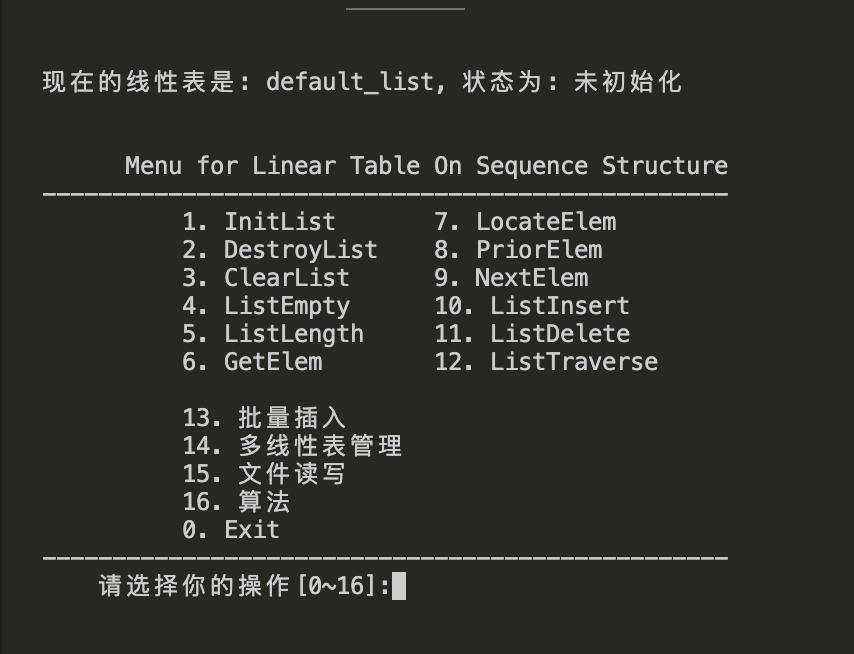
\includegraphics[width=2.5in]{sq_list/initial_interface.png}
	\caption{初始界面}
	\label{fig1-1}
\end{figure}

\subsubsection{线性表操作}

\subparagraph{InitList}
\noindent
在初始界面中输入1, 执行InitList操作, 成功时如图所示
\begin{figure}[htbp]
	\centering
	\subfloat{
		\centering
		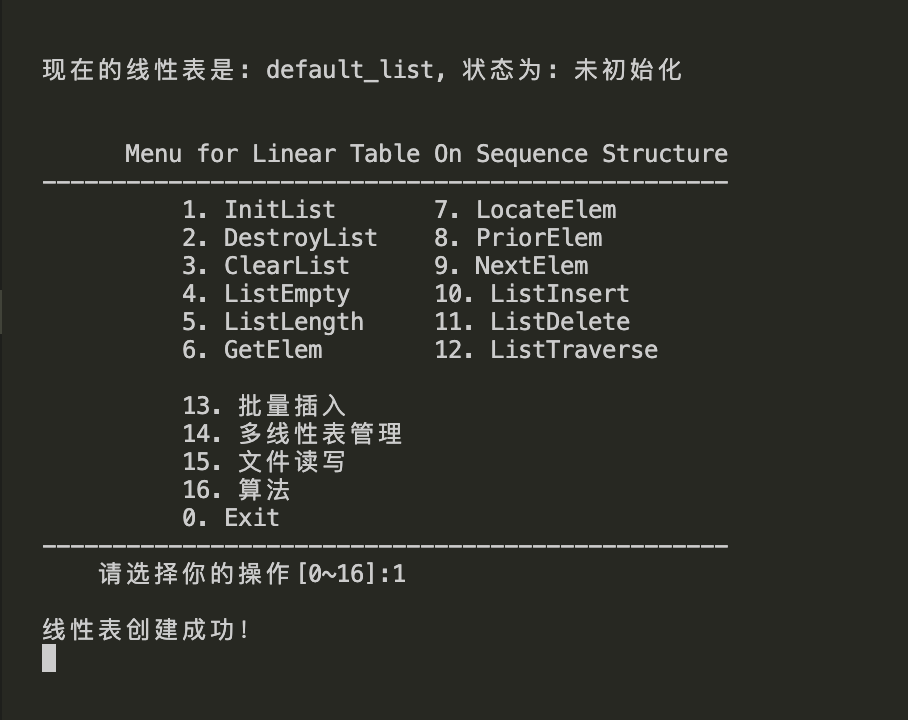
\includegraphics[width=2.3in]{sq_list/basic/InitList/InitList.png}
	}
	\centering
	\subfloat{
		\centering
		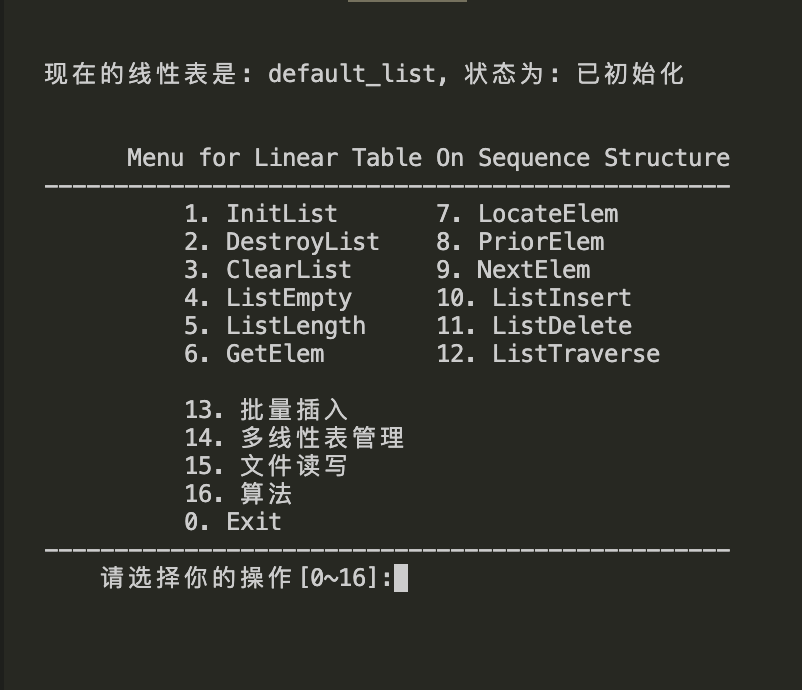
\includegraphics[width=2.3in]{sq_list/basic/InitList/InitList_after.png}
	} 
	\centering
	\caption{InitList成功}
	\label{fig1-2}
\end{figure}

\noindent
如果线性表已初始化, 则提示:
\begin{figure}[htbp]
	\centering
	\subfloat{
		\centering
		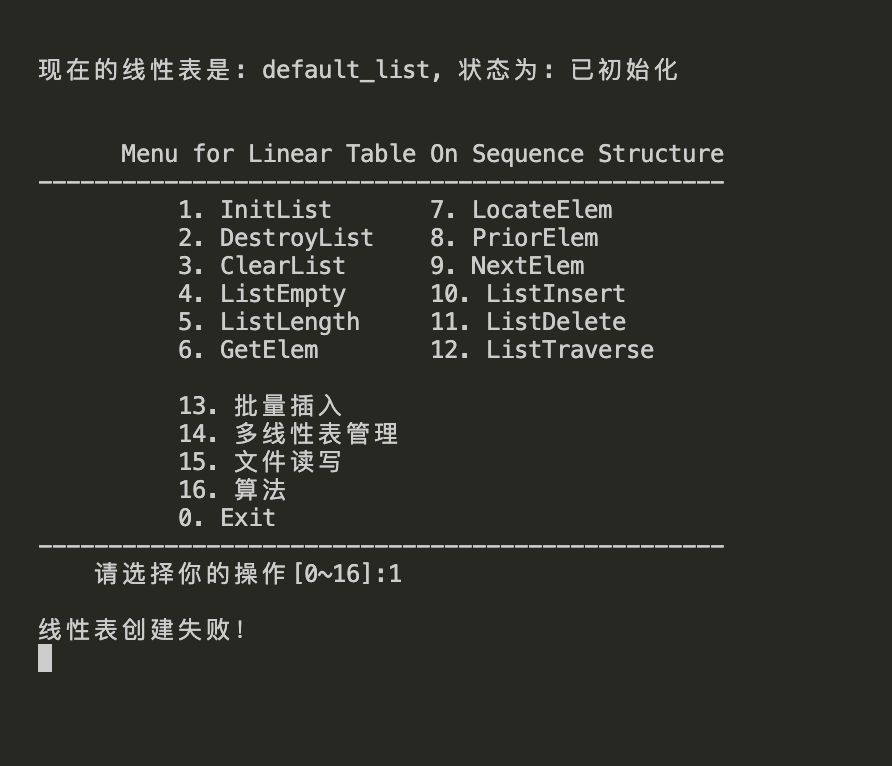
\includegraphics[width=2.3in]{sq_list/basic/InitList/InitList_infeasible.png}
	}
	\centering
	\caption{InitList失败}
	\label{fig1-2}
\end{figure}

\subparagraph{DestroyList}
\noindent
在初始界面输入2, 执行DestroyList操作, 成功时如图所示:
\begin{figure}[htbp]
	\centering
	\subfloat{
		\centering
		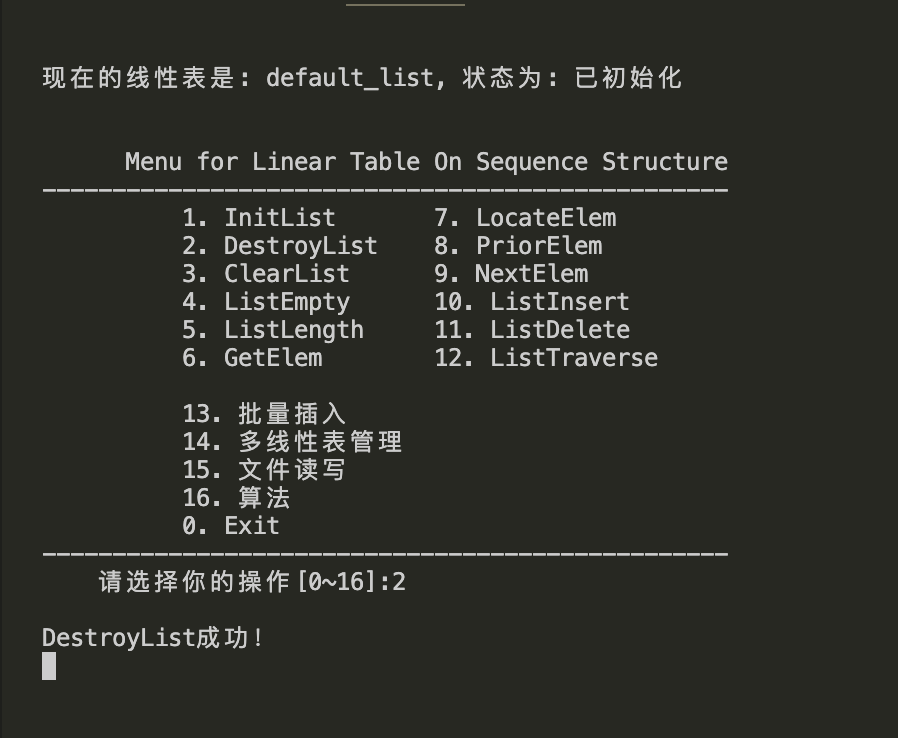
\includegraphics[width=2.3in]{sq_list/basic/DestroyList/DestroyList.png}
	}
	\centering
	\subfloat{
		\centering
		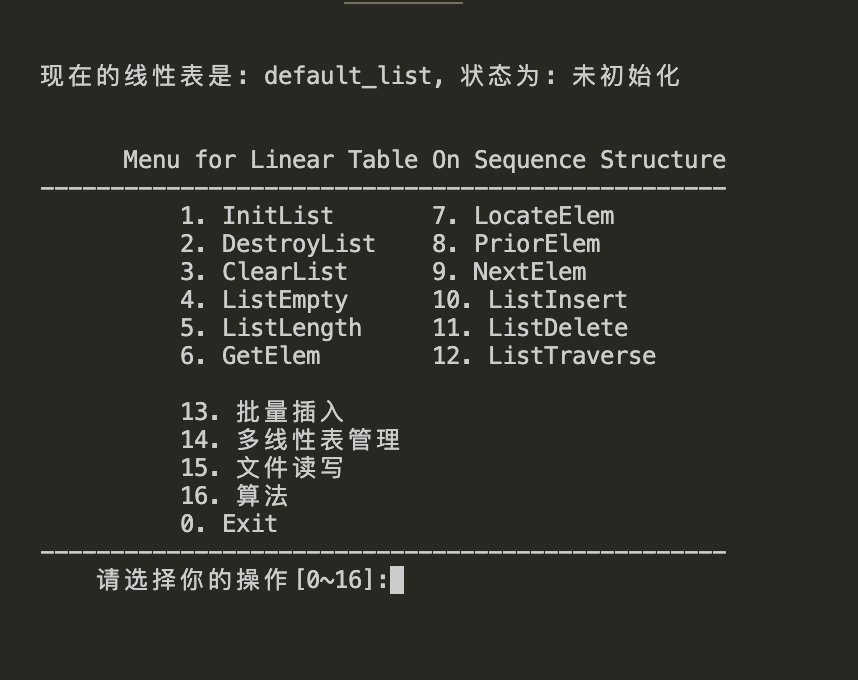
\includegraphics[width=2.3in]{sq_list/basic/DestroyList/DestroyList_after.png}
	} 
	\centering
	\caption{DestroyList成功}
	\label{fig1-3}
\end{figure}

\noindent
如果线性表未初始化, 则提示:
\begin{figure}[htbp]
	\centering
	\subfloat{
		\centering
		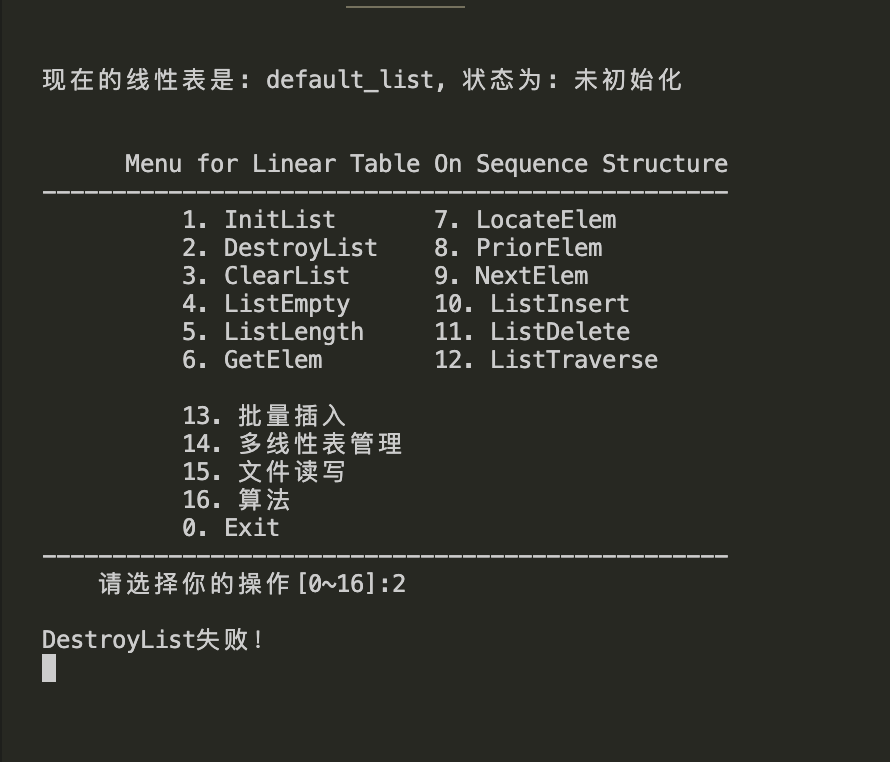
\includegraphics[width=2.3in]{sq_list/basic/DestroyList/DestroyList_infeasible.png}
	}
	\centering
	\caption{InitList失败}
	\label{fig1-4}
\end{figure}

\subparagraph{ListEmpty}
\noindent
首先创建一个空表:
\begin{figure}[htbp]
	\centering
	\subfloat{
		\centering
		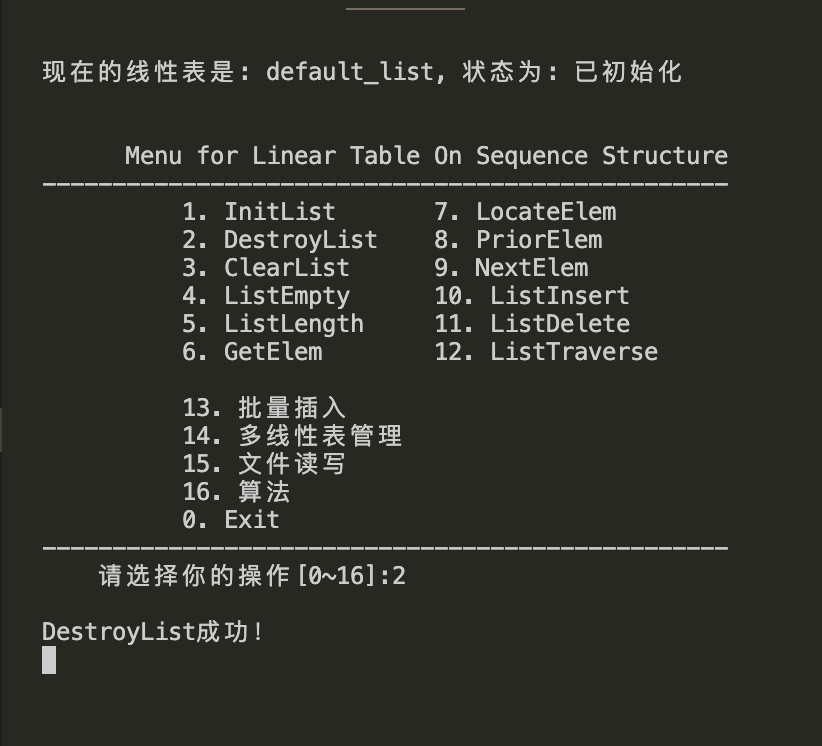
\includegraphics[width=2.3in]{sq_list/basic/ListEmpty/prelude1.png}
	}
	\centering
	\subfloat{
		\centering
		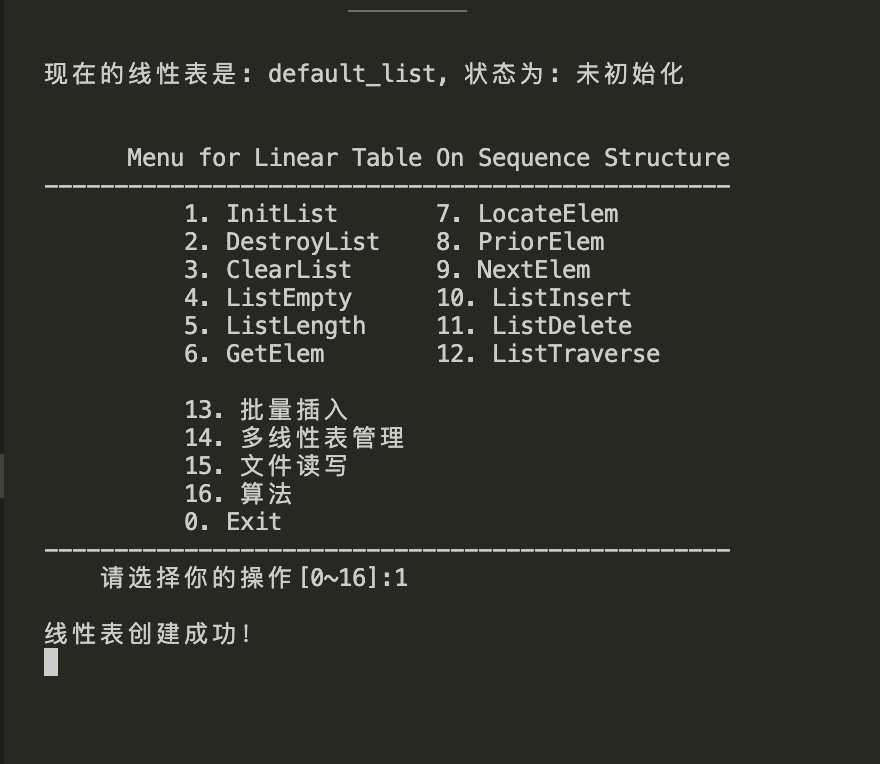
\includegraphics[width=2.3in]{sq_list/basic/ListEmpty/prelude2.png}
	} 
	\centering
	\caption{创建空表}
	\label{fig1-5}
\end{figure}

\clearpage
\noindent
然后在初始界面输入4. 输出如下:
\begin{figure}[htbp]
	\centering
	\subfloat{
		\centering
		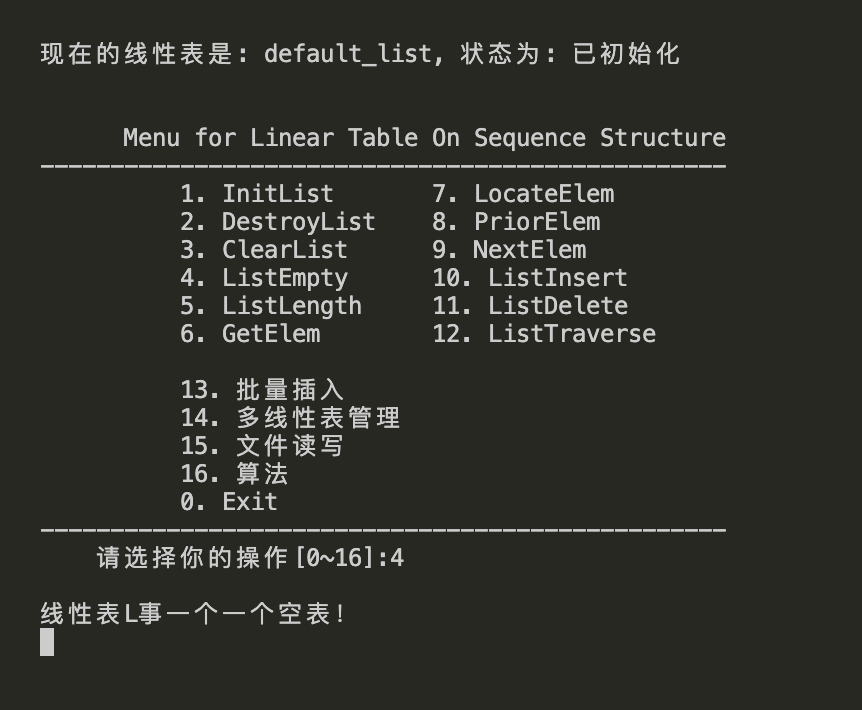
\includegraphics[width=2.3in]{sq_list/basic/ListEmpty/ok.png}
	}
	\centering
	\caption{线性表是空表}
	\label{fig1-6}
\end{figure}

\noindent
接着插入一些元素(用到了自己增加的"批量插入"功能):
\begin{figure}[htbp]
	\centering
	\subfloat{
		\centering
		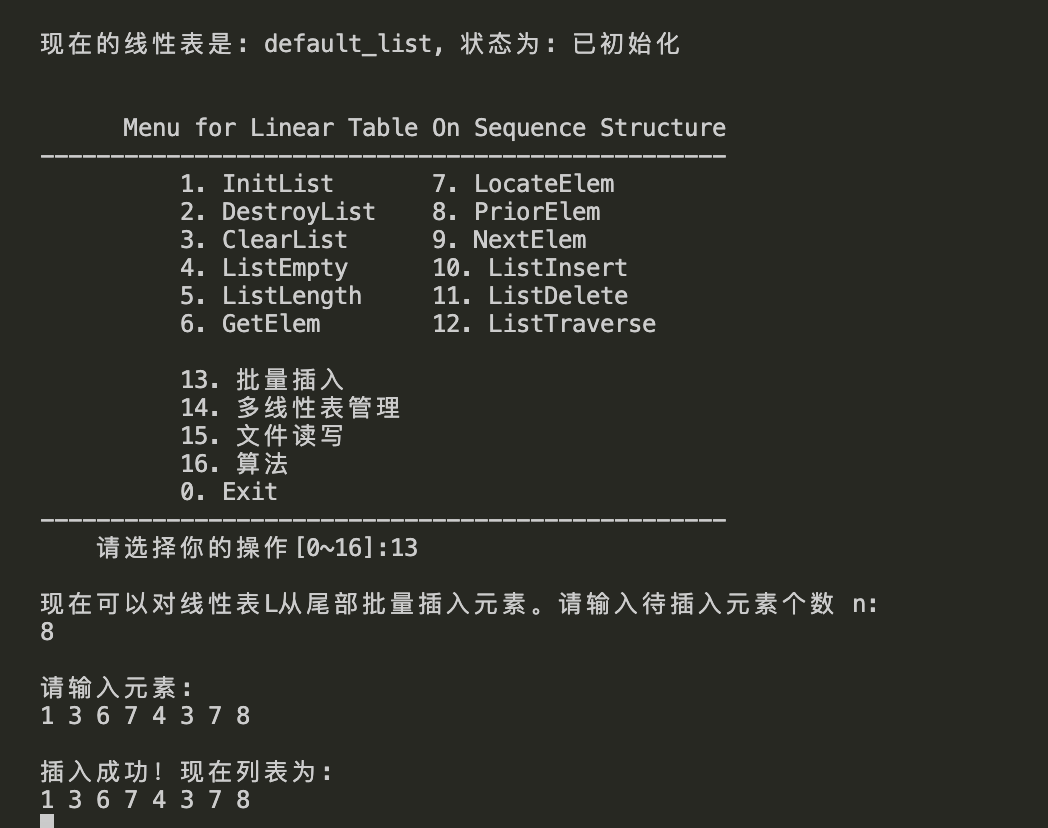
\includegraphics[width=2.3in]{sq_list/basic/ListEmpty/prelude3.png}
	}
	\centering
	\caption{插入元素}
	\label{fig1-7}
\end{figure}

\noindent
然后执行功能4:
\begin{figure}[htbp]
	\centering
	\subfloat{
		\centering
		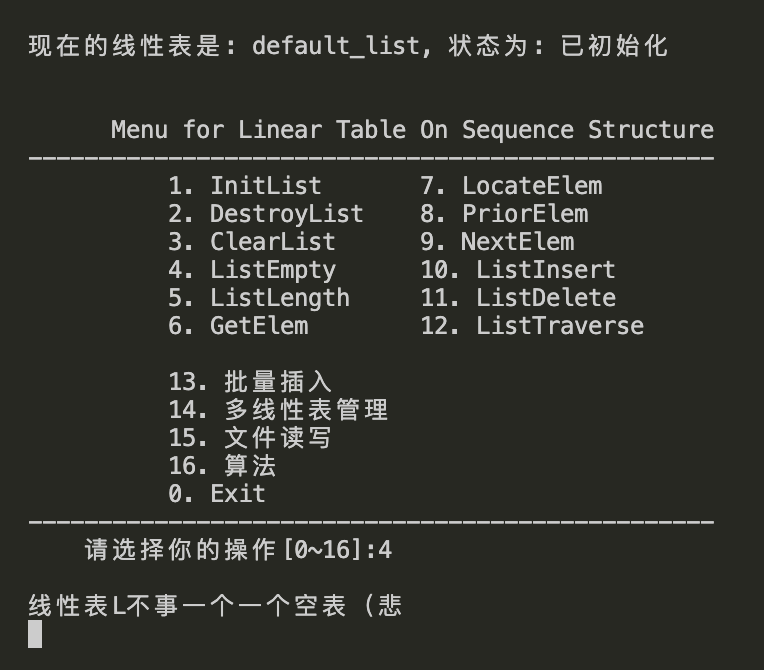
\includegraphics[width=2.3in]{sq_list/basic/ListEmpty/error.png}
	}
	\centering
	\caption{线性表不是空表}
	\label{fig1-8}
\end{figure}

\clearpage
\noindent
对于线性表未初始化的情况:
\begin{figure}[htbp]
	\centering
	\subfloat{
		\centering
		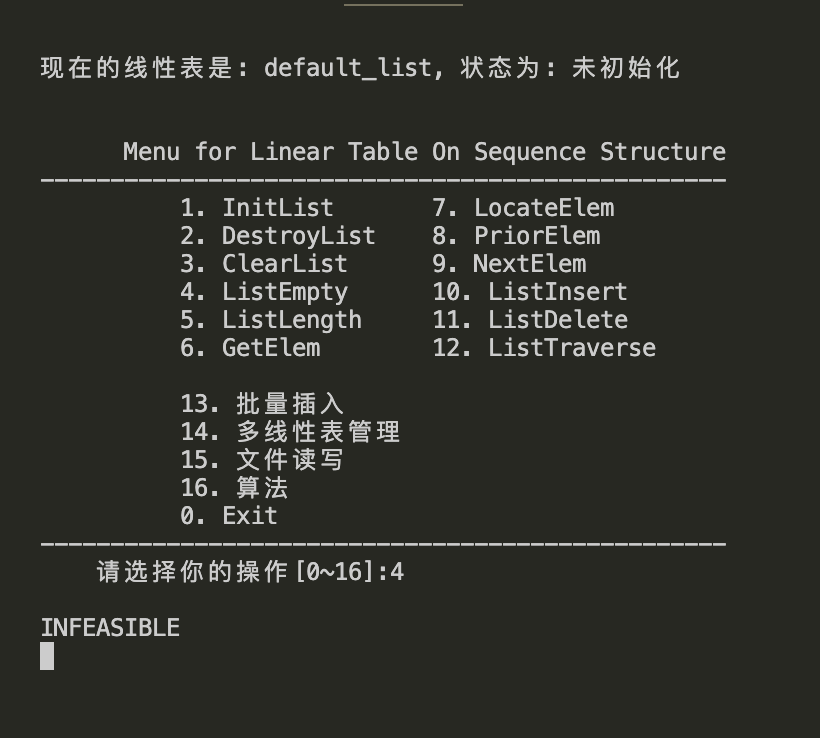
\includegraphics[width=2.3in]{sq_list/basic/ListEmpty/infeasible.png}
	}
	\centering
	\caption{插入元素}
	\label{fig1-9}
\end{figure}

\subparagraph{ClearList}
\noindent
首先创建一个空表, 并插入元素:
\begin{figure}[htbp]
	\centering
	\subfloat{
		\centering
		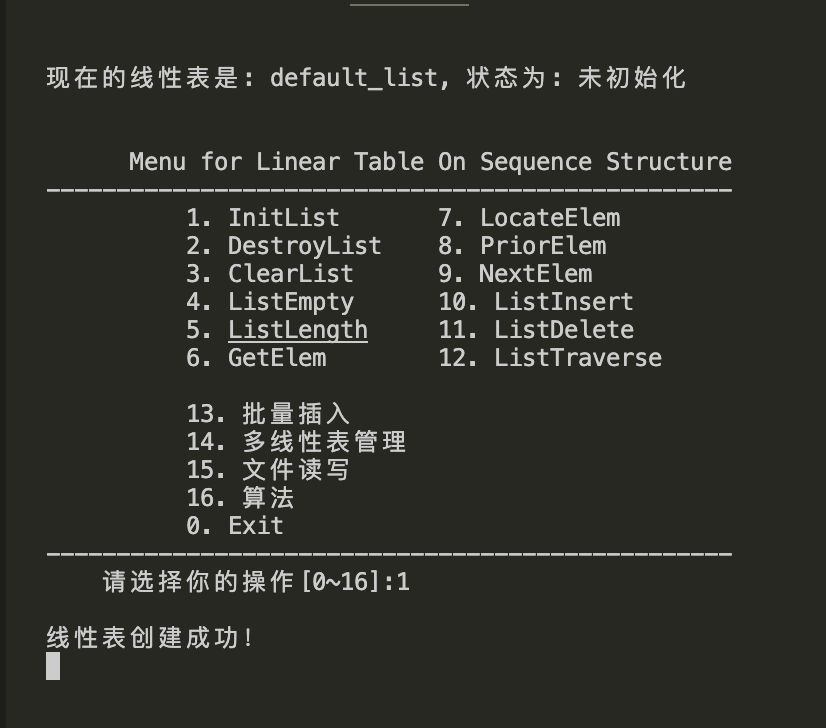
\includegraphics[width=2.1in]{sq_list/basic/ClearList/prelude1.png}
	}
	\centering
	\subfloat{
		\centering
		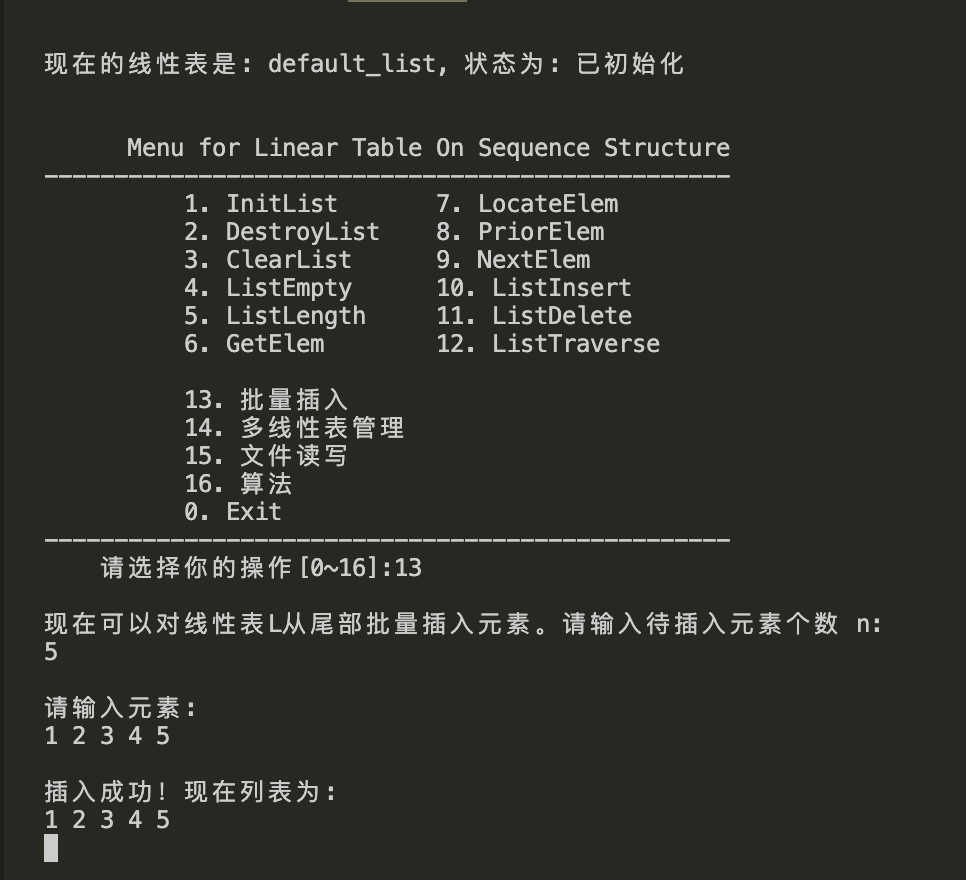
\includegraphics[width=2.1in]{sq_list/basic/ClearList/prelude2.png}
	} 
	\centering
	\caption{初始}
	\label{fig1-10}
\end{figure}

\noindent
然后在初始界面输入3, 执行ClearList操作, 成功时如图所示:
\begin{figure}[htbp]
	\centering
	\subfloat{
		\centering
		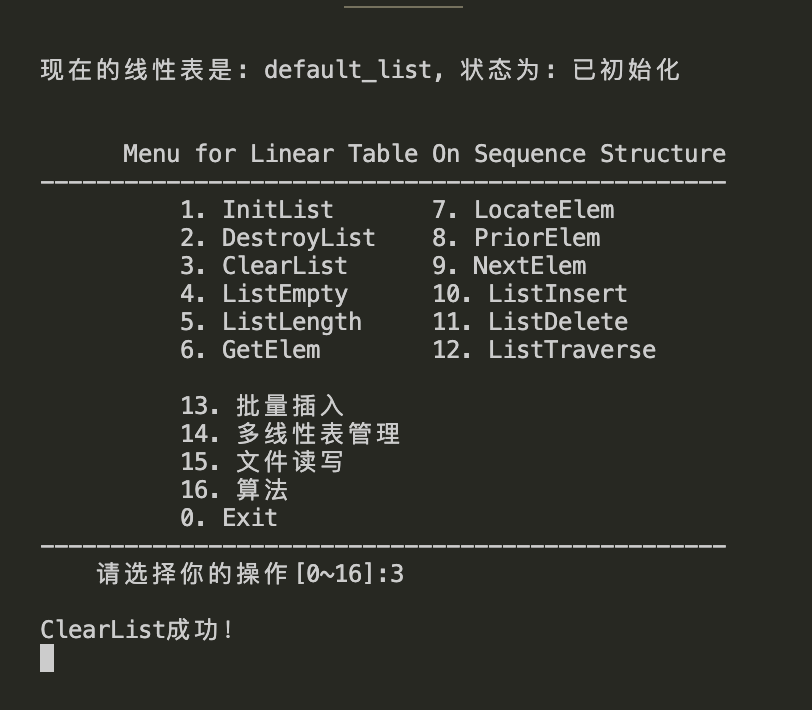
\includegraphics[width=2.1in]{sq_list/basic/ClearList/clear_list.png}
	}
	\centering
	\subfloat{
		\centering
		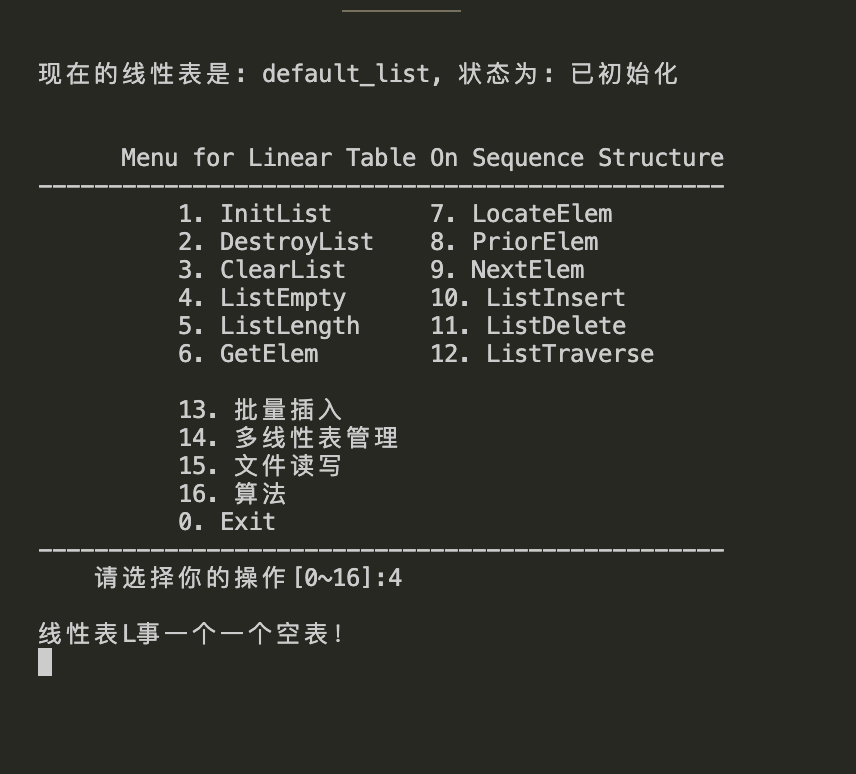
\includegraphics[width=2.1in]{sq_list/basic/ClearList/clear_list_after.png}
	} 
	\centering
	\caption{ClearList成功}
	\label{fig1-11}
\end{figure}

\clearpage
\noindent
现在执行InitList操作, 失败, 符合ClearList的语义.
\begin{figure}[htbp]
	\centering
	\subfloat{
		\centering
		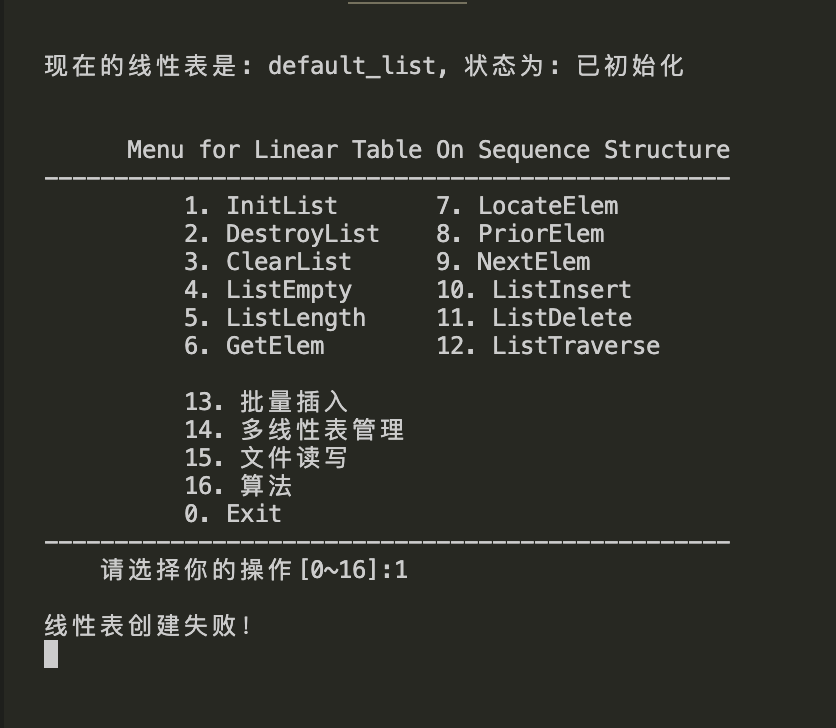
\includegraphics[width=2.3in]{sq_list/basic/ClearList/init_after_clear.png}
	}
	\centering
	\caption{ClearList失败}
	\label{fig1-12}
\end{figure}

\noindent
现在表是空表. 再执行一遍功能3:
\begin{figure}[htbp]
	\centering
	\subfloat{
		\centering
		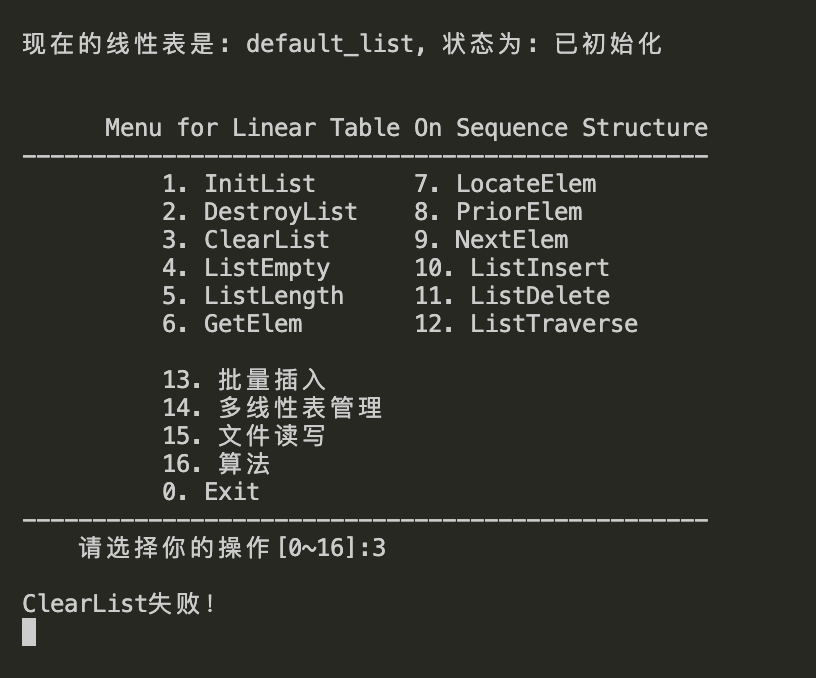
\includegraphics[width=2.3in]{sq_list/basic/ClearList/error.png}
	}
	\centering
	\caption{ClearList失败}
	\label{fig1-13}
\end{figure}

\noindent
对未初始化的线性表进行操作:
\begin{figure}[htbp]
	\centering
	\subfloat{
		\centering
		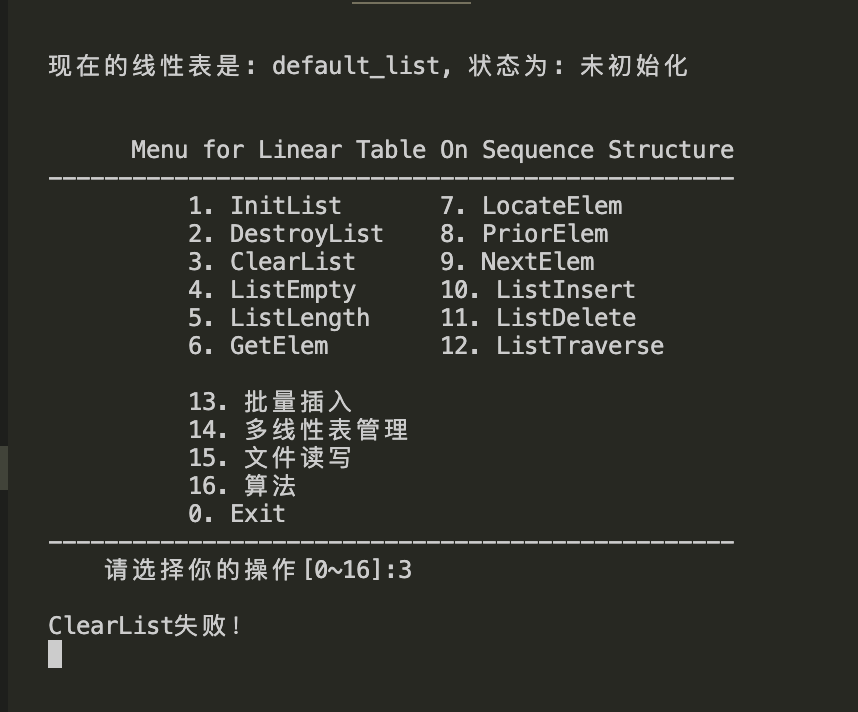
\includegraphics[width=2.3in]{sq_list/basic/ClearList/infeasible.png}
	}
	\centering
	\caption{INFEASIBLE}
	\label{fig1-14}
\end{figure}

\clearpage
\subparagraph{ListLength}
\noindent
首先创建一个空表:
\begin{figure}[htbp]
	\centering
	\subfloat{
		\centering
		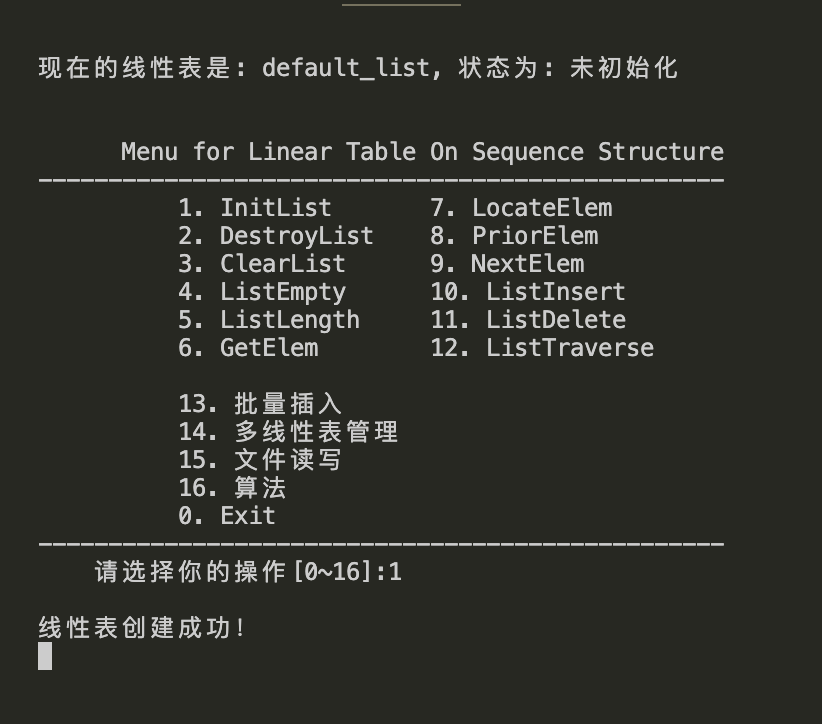
\includegraphics[width=2.1in]{sq_list/basic/ListLength/prelude1.png}
	}
	\centering
	\caption{初始}
	\label{fig1-15}
\end{figure}

\noindent
然后执行操作5. 现在表是空表.
\begin{figure}[htbp]
	\centering
	\subfloat{
		\centering
		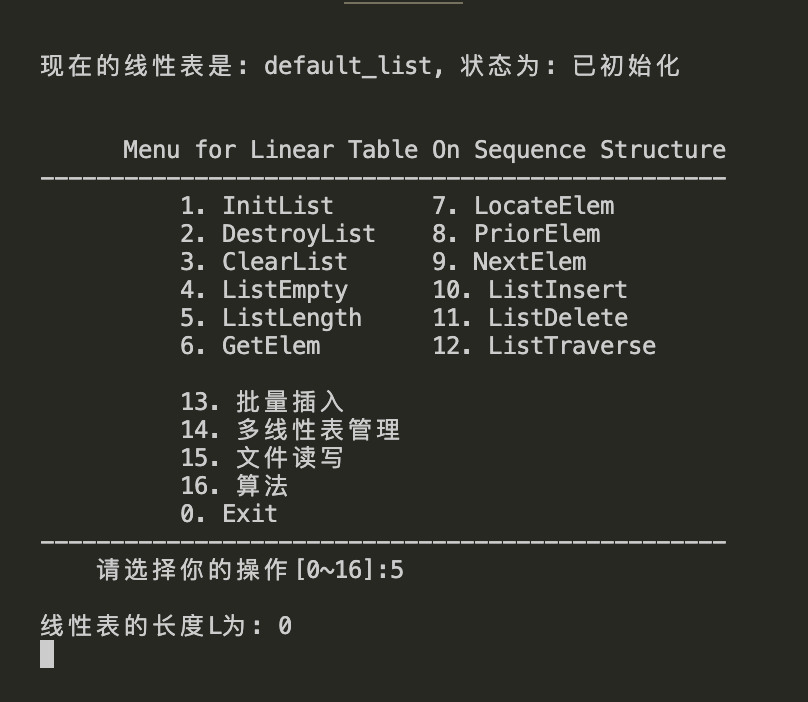
\includegraphics[width=2.1in]{sq_list/basic/ListLength/empty_list.png}
	}
	\centering
	\caption{空表}
	\label{fig1-16}
\end{figure}

\noindent
接着添加元素:
\begin{figure}[htbp]
	\centering
	\subfloat{
		\centering
		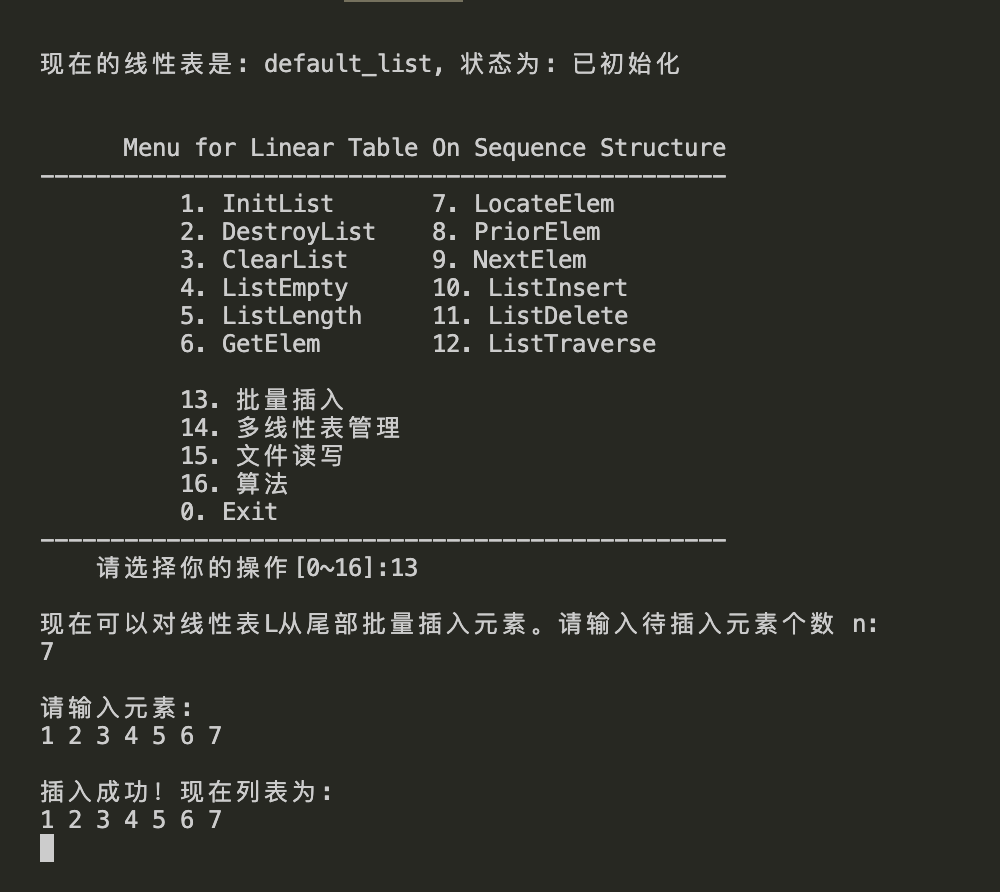
\includegraphics[width=2.1in]{sq_list/basic/ListLength/prelude2.png}
	}
	\centering
	\caption{添加元素}
	\label{fig1-17}
\end{figure}

\clearpage
\noindent
再进行一遍操作5. 可以看到, 表长变成了7.
\begin{figure}[htbp]
	\centering
	\subfloat{
		\centering
		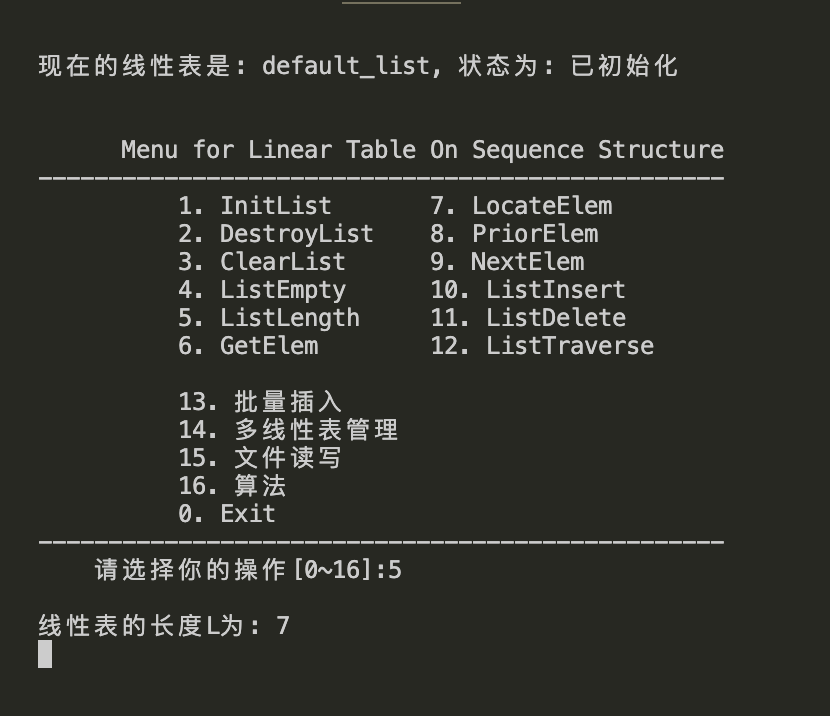
\includegraphics[width=2.1in]{sq_list/basic/ListLength/normal_list.png}
	}
	\centering
	\caption{非空的表}
	\label{fig1-18}
\end{figure}

\noindent
对未初始化的表:
\begin{figure}[htbp]
	\centering
	\subfloat{
		\centering
		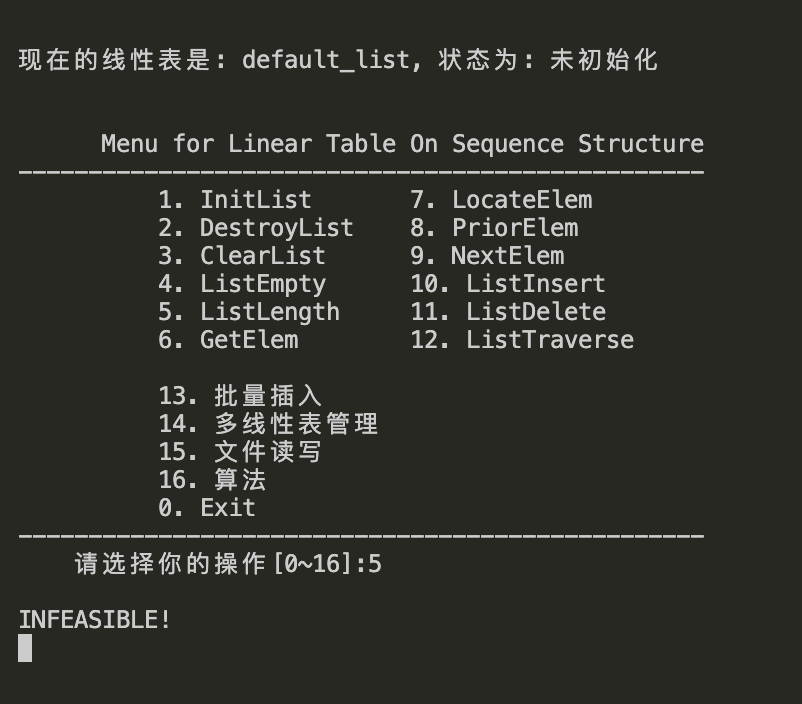
\includegraphics[width=2.1in]{sq_list/basic/ListLength/infeasible.png}
	}
	\centering
	\caption{INFEASIBLE}
	\label{fig1-19}
\end{figure}

\subparagraph{ListTraverse}
\noindent
首先创建空表并添加元素:
\begin{figure}[htbp]
	\centering
	\subfloat{
		\centering
		\includegraphics[width=2.1in]{sq_list/basic/ListTraverse/prelude1.png}
	}
	\centering
	\subfloat{
		\centering
		\includegraphics[width=2.1in]{sq_list/basic/ListTraverse/prelude2.png}
	}
	\centering
	\caption{初始}
	\label{fig1-20}
\end{figure}

\clearpage
\noindent
然后执行操作12:
\begin{figure}[htbp]
	\centering
	\subfloat{
		\centering
		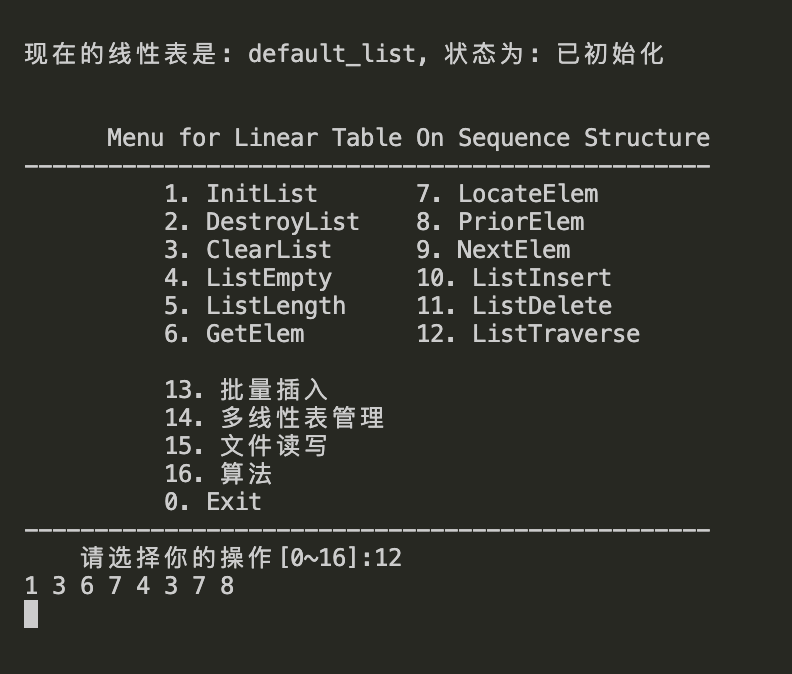
\includegraphics[width=2.1in]{sq_list/basic/ListTraverse/ok.png}
	}
	\centering
	\caption{ListTraverse成功}
	\label{fig1-21}
\end{figure}

\subparagraph{GetElem}
\noindent
首先创建空表并添加元素:
\begin{figure}[htbp]
	\centering
	\subfloat{
		\centering
		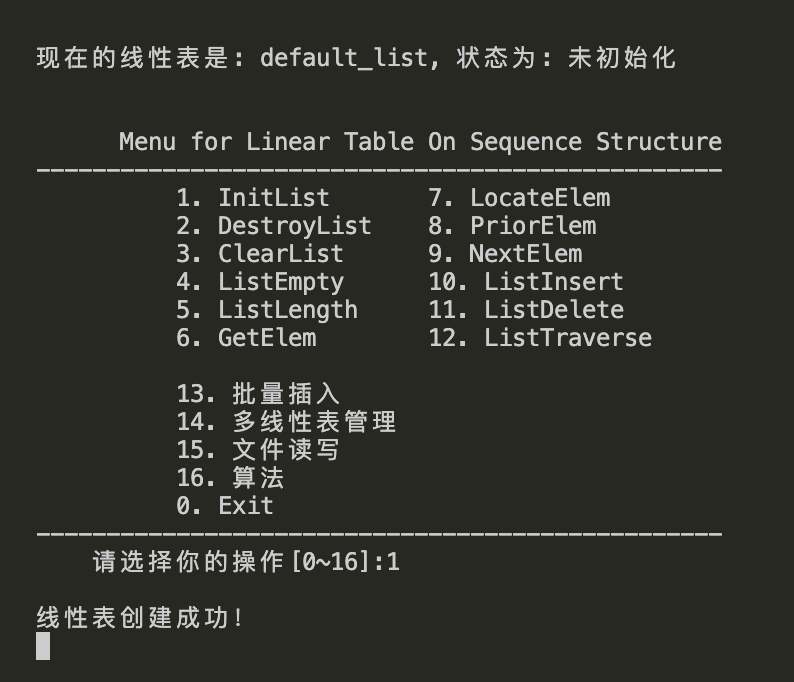
\includegraphics[width=2.1in]{sq_list/basic/GetElem/prelude1.png}
	}
	\centering
	\subfloat{
		\centering
		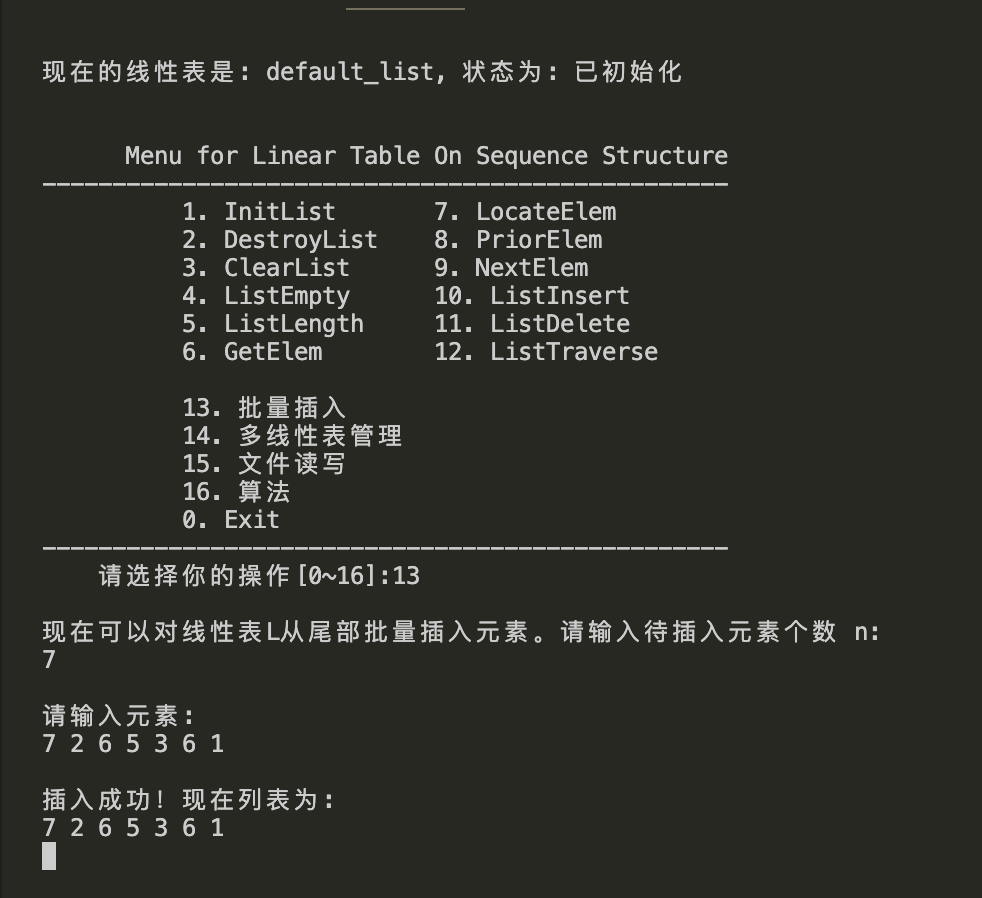
\includegraphics[width=2.1in]{sq_list/basic/GetElem/prelude2.png}
	}
	\centering
	\caption{初始}
	\label{fig1-22}
\end{figure}

\noindent
然后执行操作6. 可以看到, 操作界面输出了对应位置的元素值.
\begin{figure}[htbp]
	\centering
	\subfloat{
		\centering
		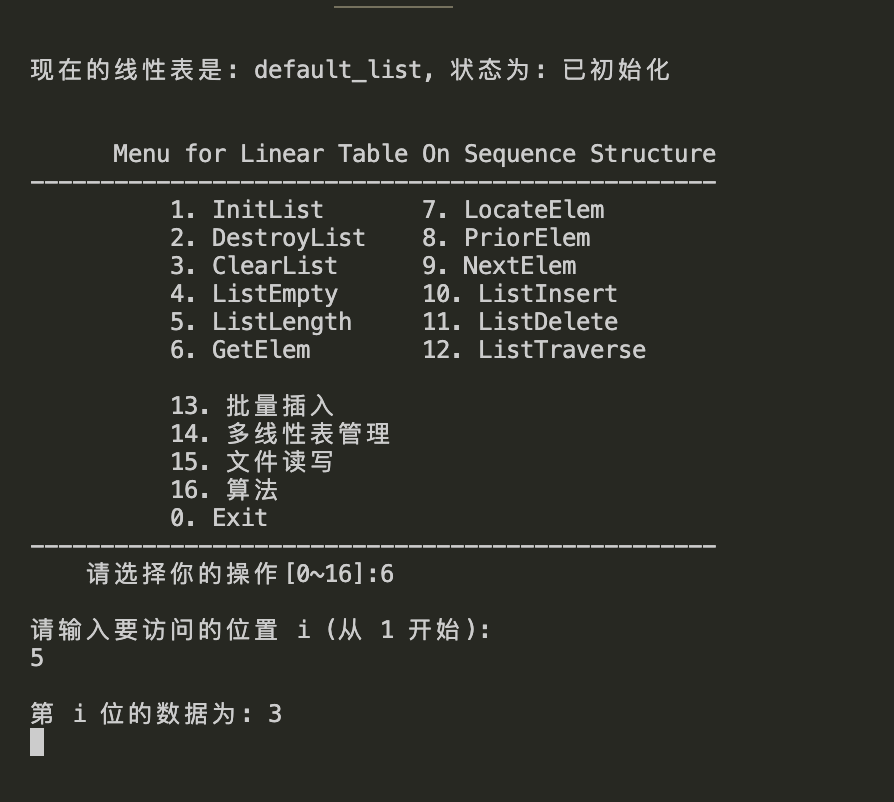
\includegraphics[width=2.1in]{sq_list/basic/GetElem/ok.png}
	}
	\centering
	\caption{GetElem成功}
	\label{fig1-23}
\end{figure}

\clearpage
\noindent
下面输入一个越界的数据, 操作界面提示了一个错误.
\begin{figure}[htbp]
	\centering
	\subfloat{
		\centering
		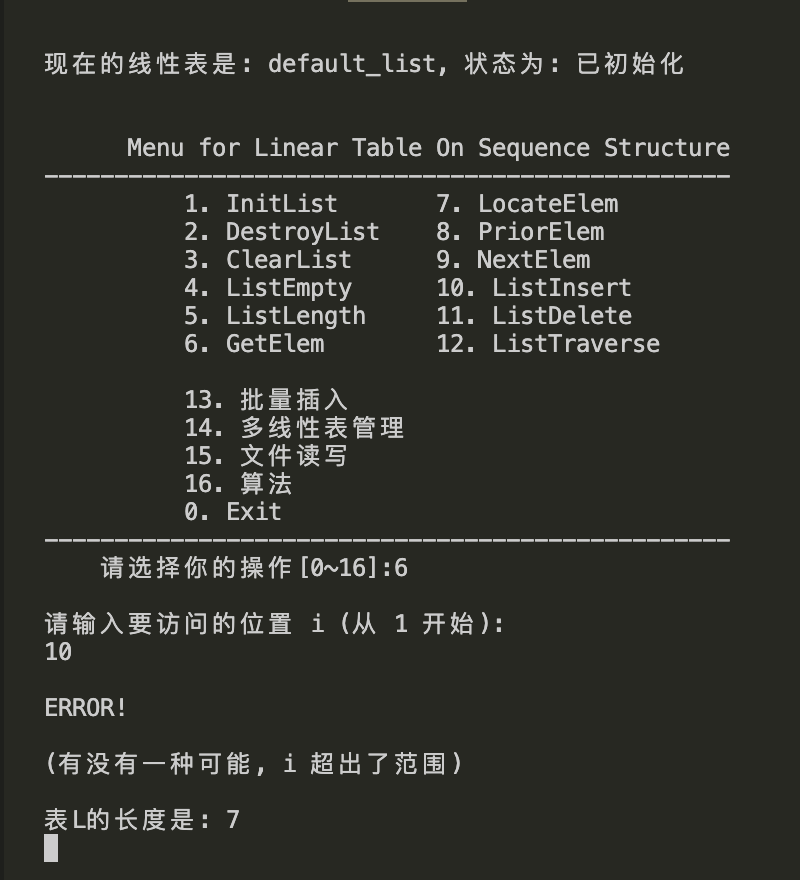
\includegraphics[width=2.1in]{sq_list/basic/GetElem/error.png}
	}
	\centering
	\caption{GetElem失败}
	\label{fig1-24}
\end{figure}

\noindent
对未初始化的线性表进行操作:
\begin{figure}[htbp]
	\centering
	\subfloat{
		\centering
		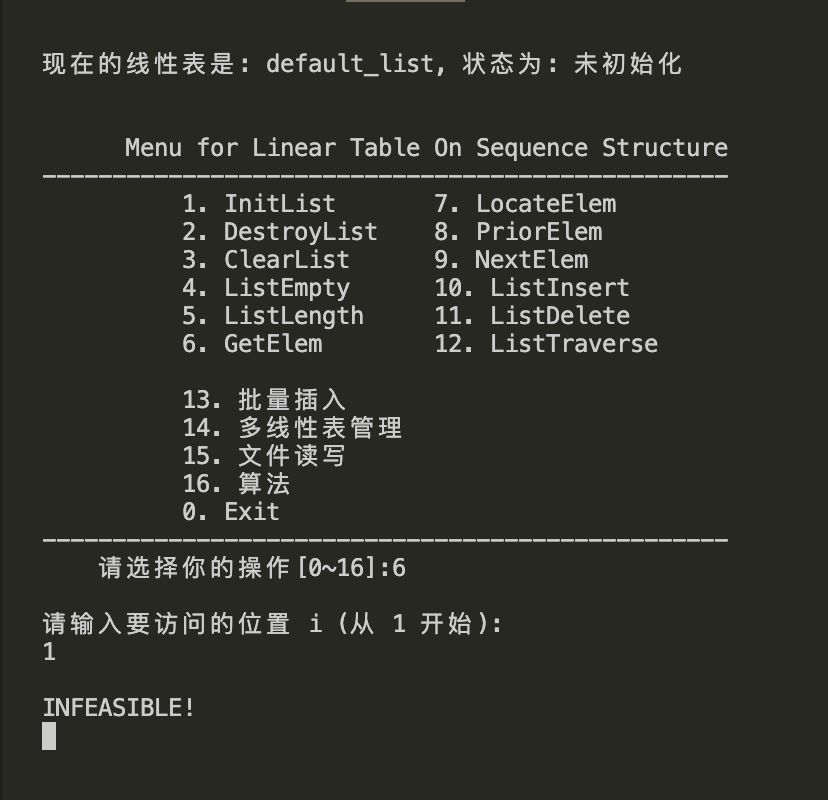
\includegraphics[width=2.1in]{sq_list/basic/GetElem/infeasible.png}
	}
	\centering
	\caption{INFEASIBLE}
	\label{fig1-25}
\end{figure}

\clearpage
\subparagraph{LocateElem}
\noindent
首先创建空表并添加元素:
\begin{figure}[htbp]
	\centering
	\subfloat{
		\centering
		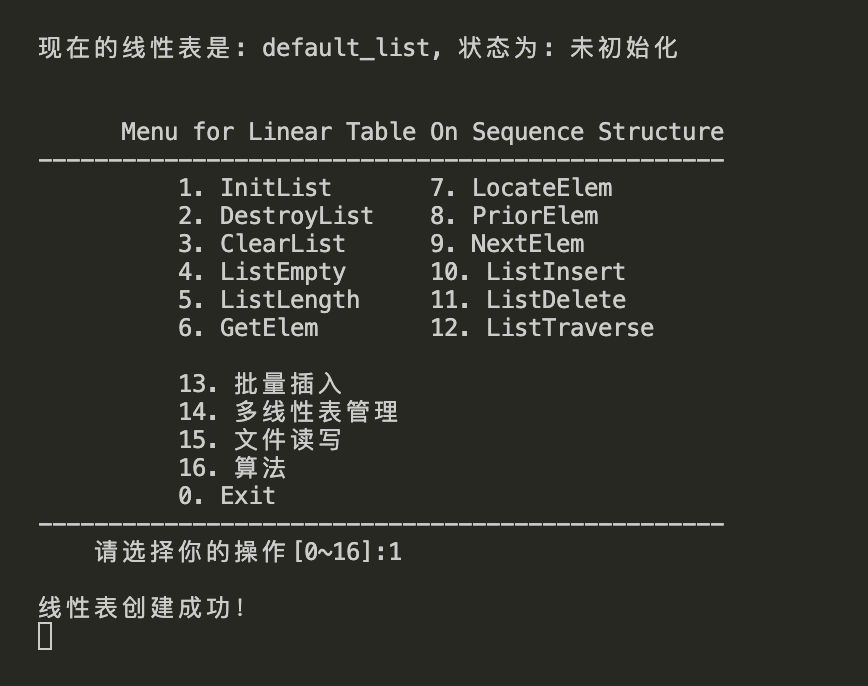
\includegraphics[width=2.2in]{sq_list/basic/LocateElem/prelude1.png}
	}
	\centering
	\subfloat{
		\centering
		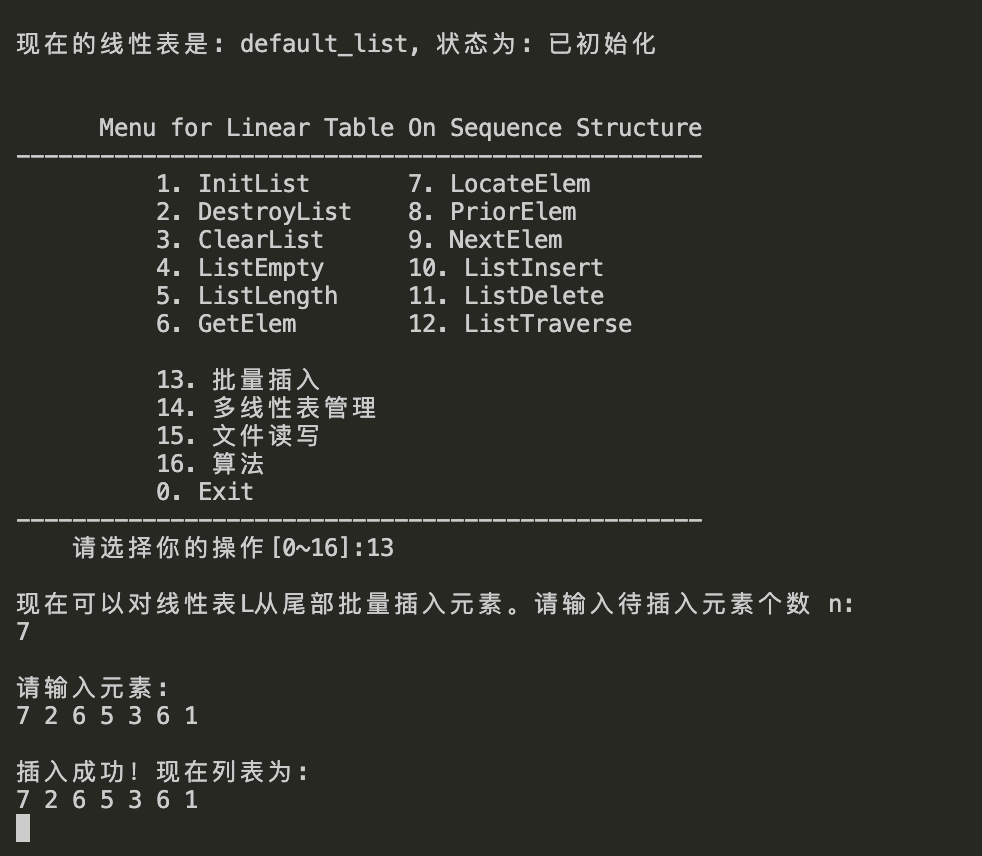
\includegraphics[width=2.2in]{sq_list/basic/LocateElem/prelude2.png}
	}
	\centering
	\caption{初始}
	\label{fig1-26}
\end{figure}

\noindent
下面输入一个只出现过一次的数据, 操作界面输出它的位置.
\begin{figure}[htbp]
	\centering
	\subfloat{
		\centering
		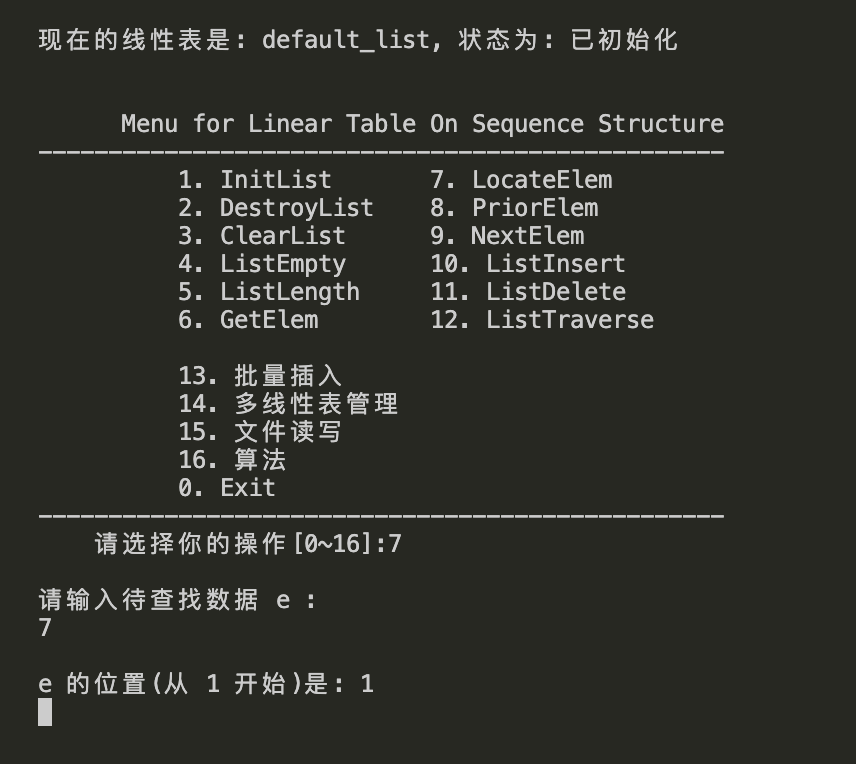
\includegraphics[width=2.1in]{sq_list/basic/LocateElem/ok_unique.png}
	}
	\centering
	\caption{LocateElem成功\_1}
	\label{fig1-27}
\end{figure}

\noindent
下面输入一个重复出现的数据, 操作界面输出它第一次出现的位置.
\begin{figure}[htbp]
	\centering
	\subfloat{
		\centering
		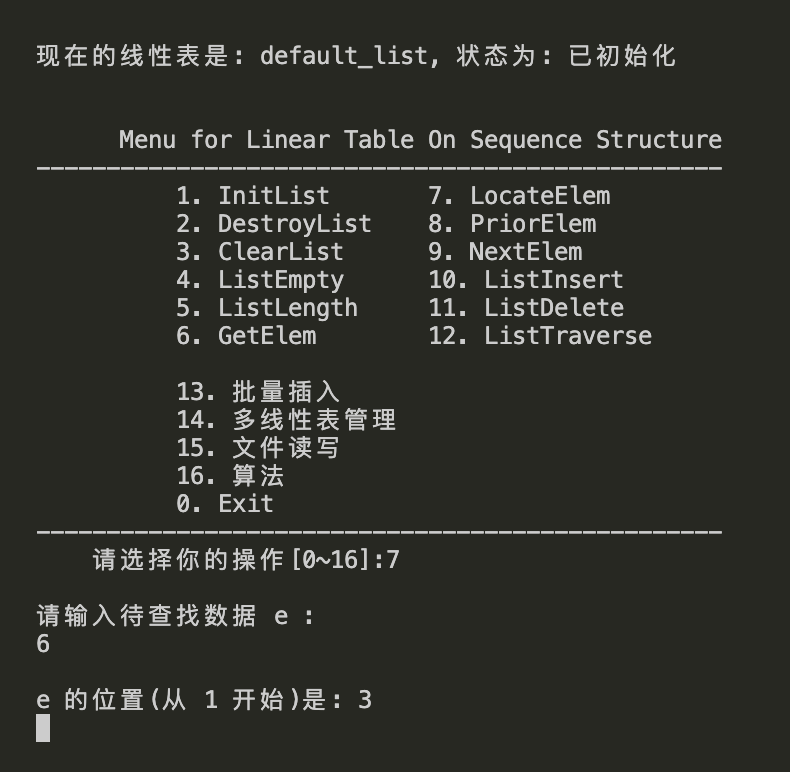
\includegraphics[width=2.1in]{sq_list/basic/LocateElem/ok_repeated.png}
	}
	\centering
	\caption{LocateElem成功\_2}
	\label{fig1-28}
\end{figure}

\clearpage
\noindent
下面输入一个表中没有的数据, 操作界面提示错误.
\begin{figure}[htbp]
	\centering
	\subfloat{
		\centering
		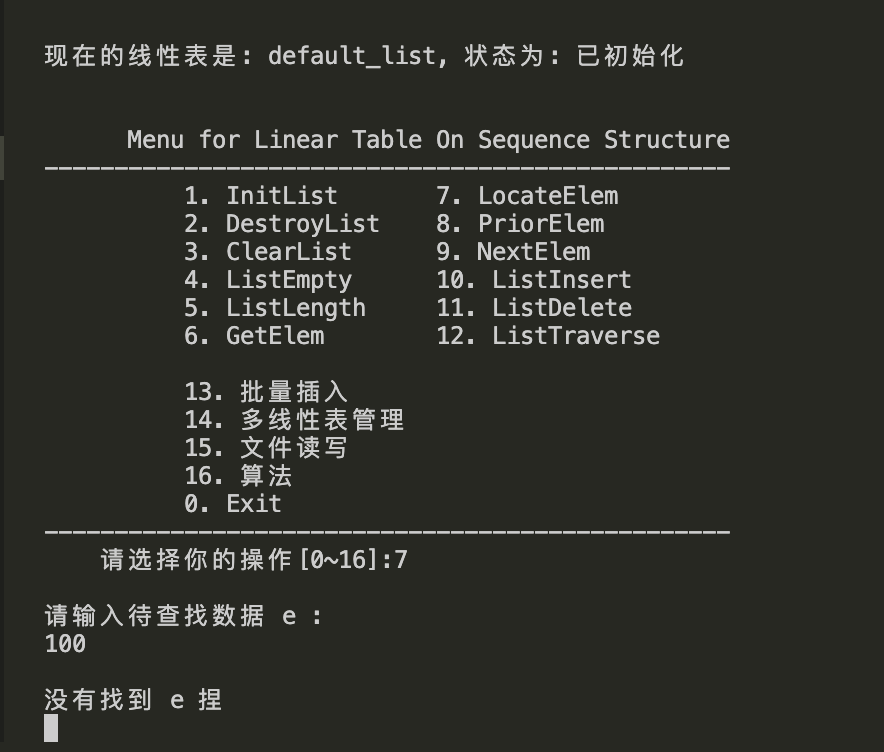
\includegraphics[width=2.1in]{sq_list/basic/LocateElem/error.png}
	}
	\centering
	\caption{LocateElem失败}
	\label{fig1-29}
\end{figure}

\noindent
线性表未初始化时:
\begin{figure}[htbp]
	\centering
	\subfloat{
		\centering
		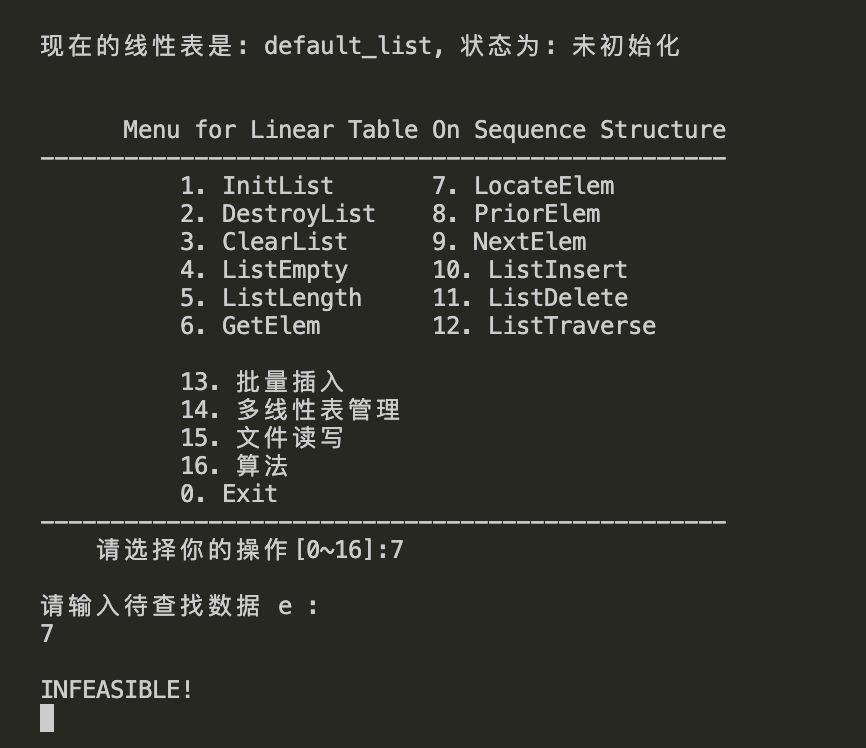
\includegraphics[width=2.1in]{sq_list/basic/LocateElem/infeasible.png}
	}
	\centering
	\caption{INFEASIBLE}
	\label{fig1-30}
\end{figure}

\subparagraph{PriorElem}
\noindent
首先创建空表并添加元素:
\begin{figure}[htbp]
	\centering
	\subfloat{
		\centering
		\includegraphics[width=2.2in]{sq_list/basic/PriorElem/prelude1.png}
	}
	\centering
	\subfloat{
		\centering
		\includegraphics[width=2.2in]{sq_list/basic/PriorElem/prelude2.png}
	}
	\centering
	\caption{初始}
	\label{fig1-31}
\end{figure}

\clearpage
\noindent
下面输入一个只出现过一次的数据, 操作界面输出它的前驱.
\begin{figure}[htbp]
	\centering
	\subfloat{
		\centering
		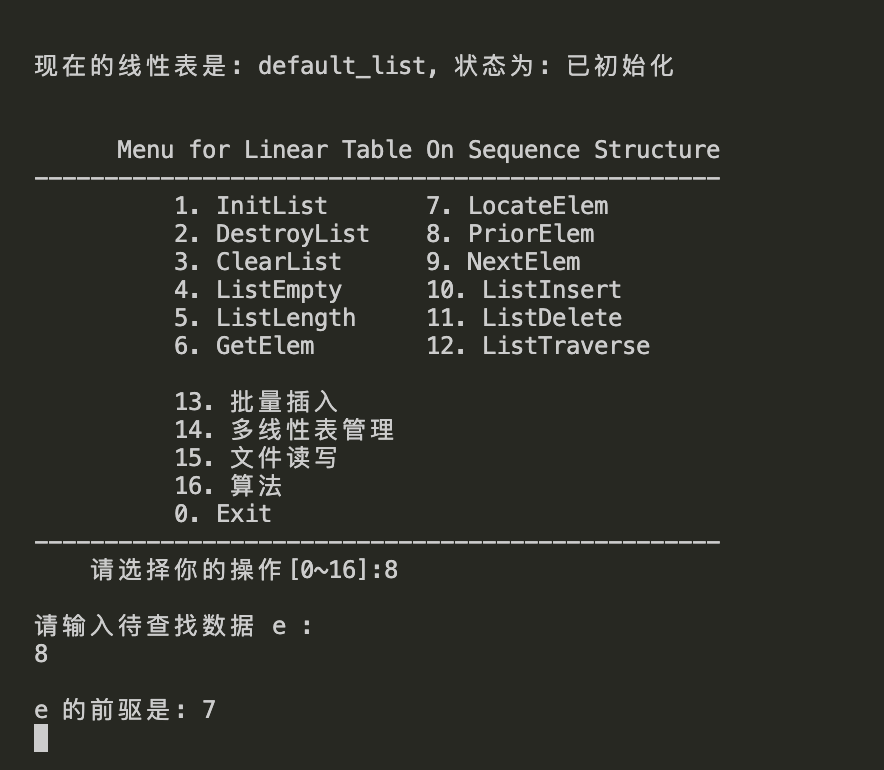
\includegraphics[width=2.2in]{sq_list/basic/PriorElem/ok_unique.png}
	}
	\centering
	\caption{PriorElem成功\_1}
	\label{fig1-32}
\end{figure}

\noindent
下面输入一个重复出现的数据, 操作界面输出它第一次出现位置的前驱元素.
\begin{figure}[htbp]
	\centering
	\subfloat{
		\centering
		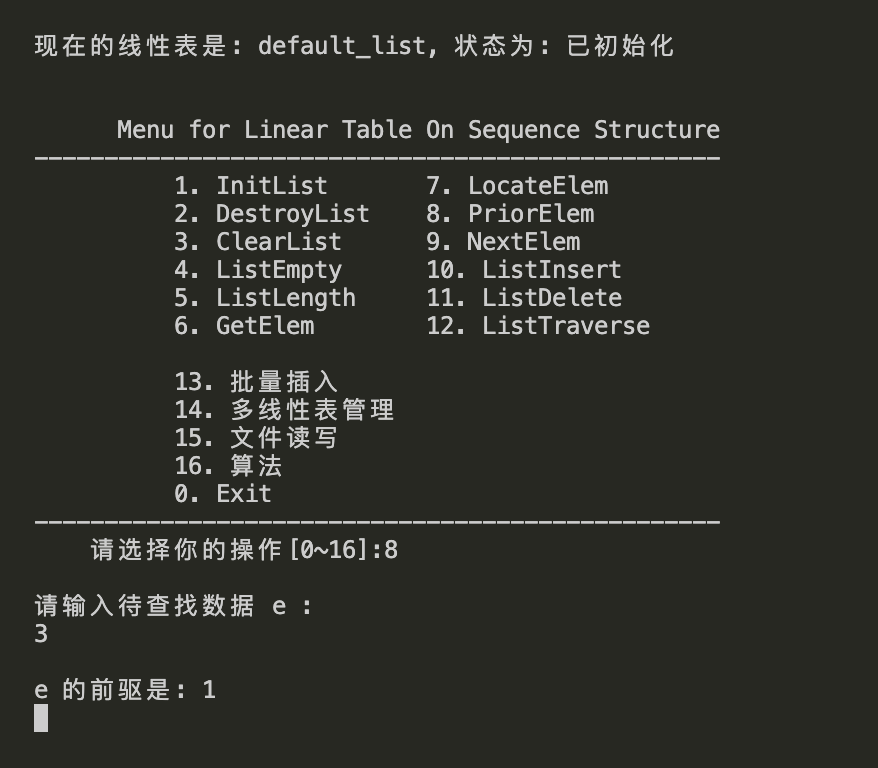
\includegraphics[width=2.1in]{sq_list/basic/PriorElem/ok_repeated.png}
	}
	\centering
	\caption{PriorElem成功\_2}
	\label{fig1-33}
\end{figure}

\noindent
下面输入一个没有前驱的数据, 操作界面提示错误.
\begin{figure}[htbp]
	\centering
	\subfloat{
		\centering
		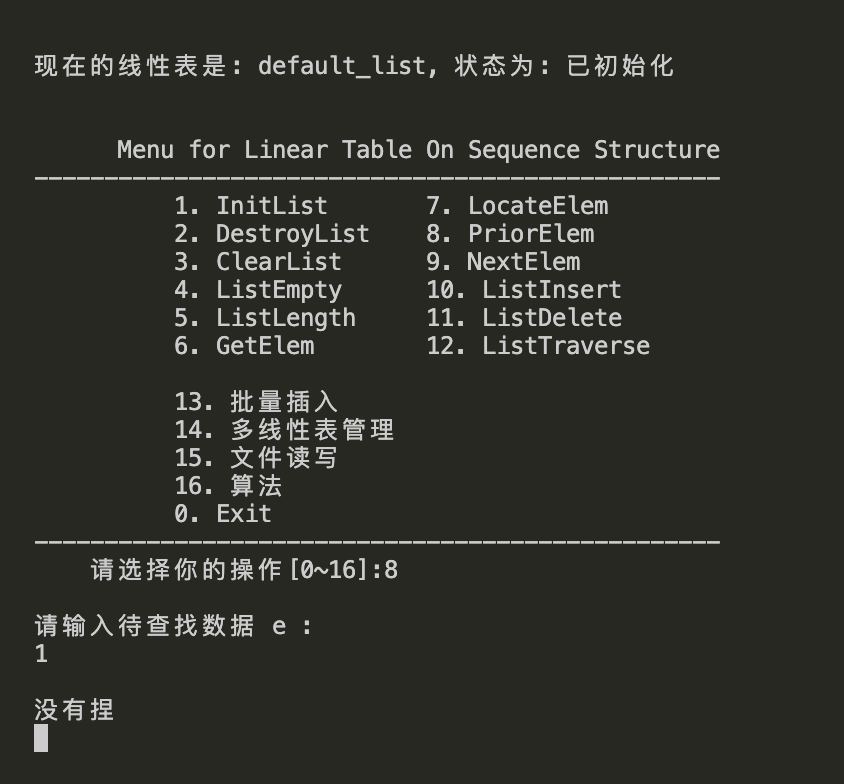
\includegraphics[width=2.1in]{sq_list/basic/PriorElem/error.png}
	}
	\centering
	\caption{PriorElem失败}
	\label{fig1-34}
\end{figure}

\clearpage
\noindent
线性表未初始化时:
\begin{figure}[htbp]
	\centering
	\subfloat{
		\centering
		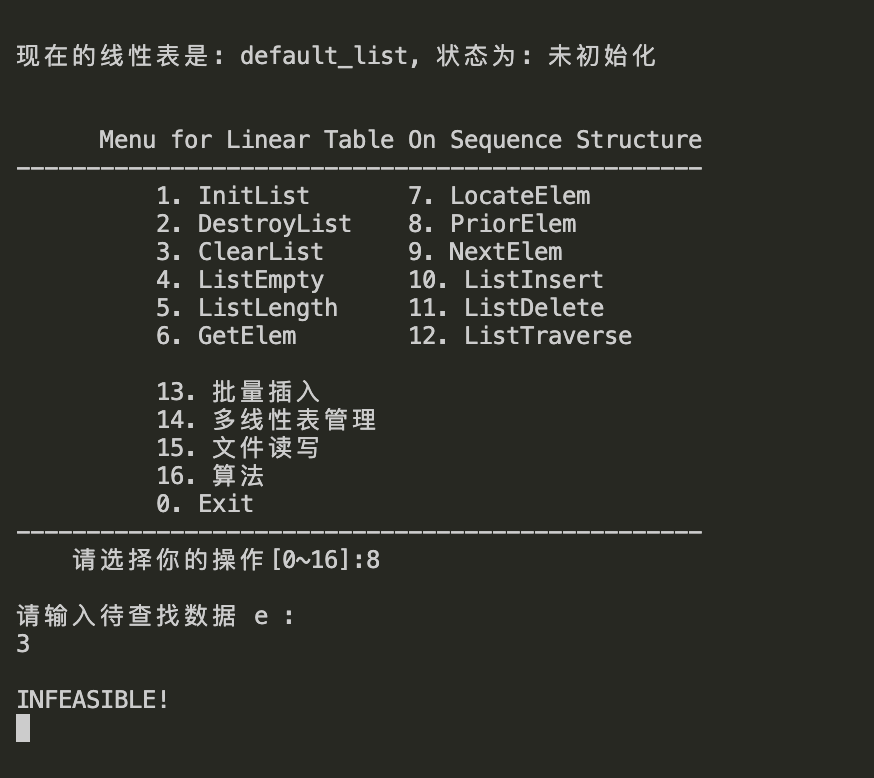
\includegraphics[width=2.1in]{sq_list/basic/PriorElem/infeasible.png}
	}
	\centering
	\caption{INFEASIBLE}
	\label{fig1-35}
\end{figure}

\subparagraph{NextElem}
\noindent
首先创建空表并添加元素:
\begin{figure}[htbp]
	\centering
	\subfloat{
		\centering
		\includegraphics[width=2.2in]{sq_list/basic/NextElem/prelude1.png}
	}
	\centering
	\subfloat{
		\centering
		\includegraphics[width=2.2in]{sq_list/basic/NextElem/prelude2.png}
	}
	\centering
	\caption{初始}
	\label{fig1-36}
\end{figure}

\noindent
下面输入一个只出现过一次的数据, 操作界面输出它的后继.
\begin{figure}[htbp]
	\centering
	\subfloat{
		\centering
		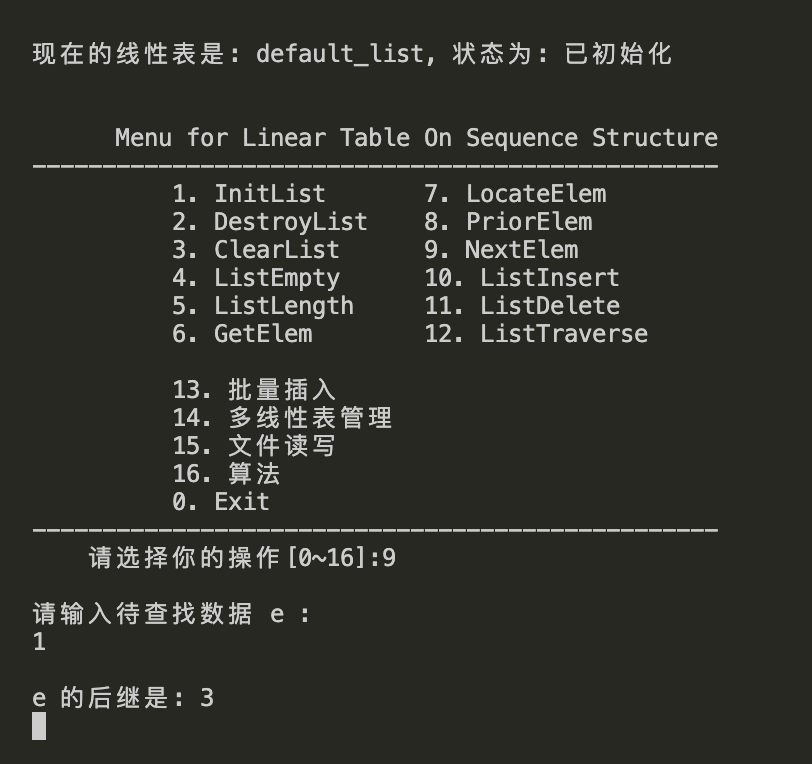
\includegraphics[width=2.2in]{sq_list/basic/NextElem/ok_unique.png}
	}
	\centering
	\caption{NextElem成功\_1}
	\label{fig1-37}
\end{figure}

\clearpage
\noindent
下面输入一个重复出现的数据, 操作界面输出它第一次出现位置的后继元素.
\begin{figure}[htbp]
	\centering
	\subfloat{
		\centering
		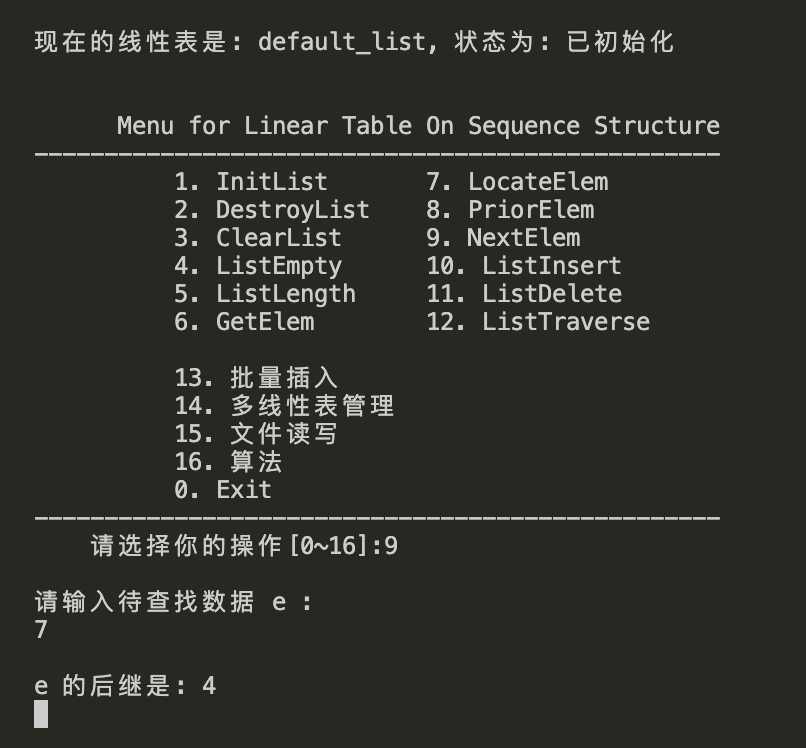
\includegraphics[width=2.1in]{sq_list/basic/NextElem/ok_repeated.png}
	}
	\centering
	\caption{NextElem成功\_2}
	\label{fig1-38}
\end{figure}

\noindent
下面输入一个没有后继的数据, 操作界面提示错误.
\begin{figure}[htbp]
	\centering
	\subfloat{
		\centering
		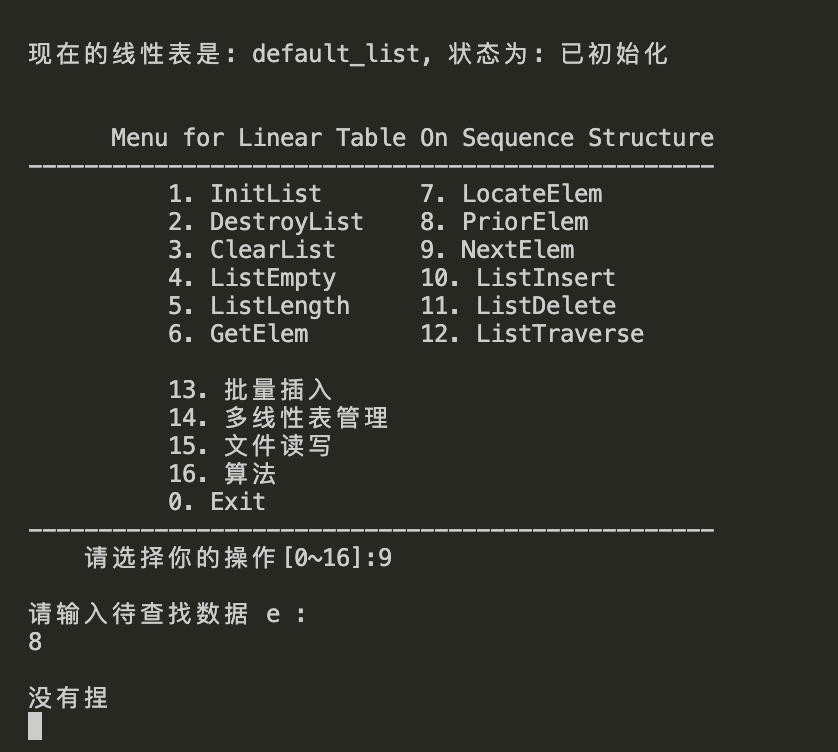
\includegraphics[width=2.1in]{sq_list/basic/NextElem/error.png}
	}
	\centering
	\caption{NextElem失败}
	\label{fig1-39}
\end{figure}

\noindent
线性表未初始化时:
\begin{figure}[htbp]
	\centering
	\subfloat{
		\centering
		\includegraphics[width=2.1in]{sq_list/basic/NextElem/infeasible.png}
	}
	\centering
	\caption{INFEASIBLE}
	\label{fig1-40}
\end{figure}

\clearpage
\subparagraph{ListInsert}
\noindent
首先创建空表并添加元素:
\begin{figure}[htbp]
	\centering
	\subfloat{
		\centering
		\includegraphics[width=2.2in]{sq_list/basic/ListInsert/prelude1.png}
	}
	\centering
	\subfloat{
		\centering
		\includegraphics[width=2.2in]{sq_list/basic/ListInsert/prelude2.png}
	}
	\centering
	\caption{初始}
	\label{fig1-41}
\end{figure}

\noindent
下面将一个元素插入到线性表的中间位置, 再进行遍历. 可以看到, 遍历的结果是正确的.
\begin{figure}[htbp]
	\centering
	\subfloat{
		\centering
		\includegraphics[width=2.2in]{sq_list/basic/ListInsert/ok1_1.png}
	}
	\subfloat{
		\centering
		\includegraphics[width=2.2in]{sq_list/basic/ListInsert/ok1_2.png}
	}
	\centering
	\caption{ListInsert成功\_1}
	\label{fig1-42}
\end{figure}

\noindent
然后将一个元素插入到线性表的末尾, 再进行遍历. 可以看到, 遍历的结果是正确的.
\begin{figure}[htbp]
	\centering
	\subfloat{
		\centering
		\includegraphics[width=2.2in]{sq_list/basic/ListInsert/ok2_1.png}
	}
	\subfloat{
		\centering
		\includegraphics[width=2.2in]{sq_list/basic/ListInsert/ok2_2.png}
	}
	\centering
	\caption{ListInsert成功\_2}
	\label{fig1-43}
\end{figure}

\clearpage
\noindent
下面将元素插入到错误的位置(分别是表的末尾以后和开头之前), 均产生错误.
\begin{figure}[htbp]
	\centering
	\subfloat{
		\centering
		\includegraphics[width=2.3in]{sq_list/basic/ListInsert/error1.png}
	}
	\subfloat{
		\centering
		\includegraphics[width=2.1in]{sq_list/basic/ListInsert/error2.png}
	}
	\centering
	\caption{ListInsert失败}
	\label{fig1-44}
\end{figure}

\noindent
线性表未初始化时:
\begin{figure}[htbp]
	\centering
	\subfloat{
		\centering
		\includegraphics[width=2.1in]{sq_list/basic/ListInsert/infeasible.png}
	}
	\centering
	\caption{INFEASIBLE}
	\label{fig1-45}
\end{figure}

\subparagraph{ListDelete}
\noindent
为方便起见, 使用ListInsert操作后的数据来测试.\\
下面删除一个线性表中间位置的元素, 再进行遍历. 可以看到, 遍历的结果是正确的.
\begin{figure}[htbp]
	\centering
	\subfloat{
		\centering
		\includegraphics[width=2.2in]{sq_list/basic/ListDelete/ok1_1.png}
	}
	\subfloat{
		\centering
		\includegraphics[width=2.2in]{sq_list/basic/ListDelete/ok1_2.png}
	}
	\centering
	\caption{ListDelete成功\_1}
	\label{fig1-46}
\end{figure}

\clearpage
\noindent
然后删除线性表末尾的元素, 再进行遍历. 可以看到, 遍历的结果是正确的.
\begin{figure}[htbp]
	\centering
	\subfloat{
		\centering
		\includegraphics[width=2.2in]{sq_list/basic/ListDelete/ok2_1.png}
	}
	\subfloat{
		\centering
		\includegraphics[width=2.2in]{sq_list/basic/ListDelete/ok2_2.png}
	}
	\centering
	\caption{ListDelete成功\_2}
	\label{fig1-47}
\end{figure}

\noindent
下面删除错误位置的元素(分别是表的末尾以后和开头之前), 均产生错误.
\begin{figure}[htbp]
	\centering
	\subfloat{
		\centering
		\includegraphics[width=2.3in]{sq_list/basic/ListDelete/error1.png}
	}
	\subfloat{
		\centering
		\includegraphics[width=2.1in]{sq_list/basic/ListDelete/error2.png}
	}
	\centering
	\caption{ListDelete失败}
	\label{fig1-48}
\end{figure}

\noindent
线性表未初始化时:
\begin{figure}[htbp]
	\centering
	\subfloat{
		\centering
		\includegraphics[width=2.1in]{sq_list/basic/ListDelete/infeasible.png}
	}
	\centering
	\caption{INFEASIBLE}
	\label{fig1-49}
\end{figure}

\newpage

\subsubsection{多线性表管理}
操作界面如下:
\begin{figure}[htbp]
	\centering
	\subfloat{
		\centering
		\includegraphics[width=2.1in]{sq_list/multi_list/interface.png}
	}
	\centering
	\caption{操作界面}
	\label{fig2-1}
\end{figure}

\subparagraph{AddList}
\noindent
首先进行操作1, 输入待添加线性表的名字ok\_computer, 操作界面显示插入成功.
\begin{figure}[htbp]
	\centering
	\subfloat{
		\centering
		\includegraphics[width=2.1in]{sq_list/multi_list/AddList/ok1_1.png}
	}
	\centering
	\caption{AddList成功}
	\label{fig2-2}
\end{figure}

\noindent
回到操作界面后, 我们发现线性表多了一个ok\_computer.
\begin{figure}[htbp]
	\centering
	\subfloat{
		\centering
		\includegraphics[width=2.1in]{sq_list/multi_list/AddList/ok1_2.png}
	}
	\centering
	\caption{AddList成功}
	\label{fig2-3}
\end{figure}

\clearpage
\subparagraph{切换线性表}
\noindent
这个功能没有做成函数, 姑且看一下吧.\\
先看一下错误情况, 即没有这个线性表:
\begin{figure}[htbp]
	\centering
	\subfloat{
		\centering
		\includegraphics[width=2.1in]{sq_list/multi_list/SwitchList/error.png}
	}
	\centering
	\caption{切换失败}
	\label{fig2-4}
\end{figure}

\noindent
如果有这个线性表, 那么切换成功. 回到操作界面以后, 星号在切换到的表上.
\begin{figure}[htbp]
	\centering
	\subfloat{
		\centering
		\includegraphics[width=2.1in]{sq_list/multi_list/SwitchList/ok1_1.png}
	}
	\subfloat{
		\centering
		\includegraphics[width=2.1in]{sq_list/multi_list/SwitchList/ok1_2.png}
	}
	\centering
	\caption{切换成功\_1}
	\label{fig2-5}
\end{figure}

\noindent
现在回到主界面, 查看我们刚刚建的新表. 很显然, 它是个空表.
\begin{figure}[htbp]
	\centering
	\subfloat{
		\centering
		\includegraphics[width=2.1in]{sq_list/multi_list/SwitchList/ok1_3.png}
	}
	\subfloat{
		\centering
		\includegraphics[width=2.1in]{sq_list/multi_list/SwitchList/ok1_4.png}
	}
	\centering
	\caption{切换成功\_2}
	\label{fig2-6}
\end{figure}

\clearpage
\noindent
现在对新表插入元素, 再切换到旧表. 遍历一遍旧表, 发现对新表的操作并不影响旧表的数据.
\begin{figure}[htbp]
	\centering
	\subfloat{
		\centering
		\includegraphics[width=2.0in]{sq_list/multi_list/SwitchList/ok1_5.png}
	}
	\centering
	\subfloat{
		\centering
		\includegraphics[width=2.0in]{sq_list/multi_list/SwitchList/ok1_6.png}
	}
	\centering
	\subfloat{
		\centering
		\includegraphics[width=2.0in]{sq_list/multi_list/SwitchList/ok1_7.png}
	}
	\centering
	\caption{切换成功\_3}
	\label{fig2-7}
\end{figure}

\subparagraph{LocateList}
\noindent
先看一下错误情况, 即没有这个线性表:
\begin{figure}[htbp]
	\centering
	\subfloat{
		\centering
		\includegraphics[width=2.5in]{sq_list/multi_list/LocateList/error.png}
	}
	\centering
	\caption{查找失败}
	\label{fig2-8}
\end{figure}

\noindent
再看一下正确情况, 即有这个线性表:
\begin{figure}[htbp]
	\centering
	\subfloat{
		\centering
		\includegraphics[width=2.5in]{sq_list/multi_list/LocateList/ok_1.png}
	}
	\centering
	\caption{查找成功}
	\label{fig2-9}
\end{figure}

\clearpage
\subparagraph{RemoveList}
\noindent
先看一下错误情况, 即没有这个线性表:
\begin{figure}[htbp]
	\centering
	\subfloat{
		\centering
		\includegraphics[width=2.5in]{sq_list/multi_list/RemoveList/error.png}
	}
	\centering
	\caption{删除失败}
	\label{fig2-10}
\end{figure}

\noindent
如果有这个线性表, 那么删除成功. \\
如果被删除的线性表就是现在正进行操作的线性表, 则删除后线性表指针切换到头一个线性表.查找、切换到原来的线性表, 均显示未找到.
\begin{figure}[htbp]
	\centering
	\subfloat{
		\centering
		\includegraphics[width=2.1in]{sq_list/multi_list/RemoveList/ok1_1.png}
	}
	\subfloat{
		\centering
		\includegraphics[width=2.1in]{sq_list/multi_list/RemoveList/ok1_2.png}
	}
	\subfloat{
		\centering
		\includegraphics[width=2.1in]{sq_list/multi_list/RemoveList/ok1_3.png}
	}
	\centering
	\caption{删除成功\_1}
	\label{fig2-11}
\end{figure}

\noindent
看一下现在的线性表. 可以看到数据不受影响.
\begin{figure}[htbp]
	\centering
	\subfloat{
		\centering
		\includegraphics[width=2.1in]{sq_list/multi_list/RemoveList/ok1_4.png}
	}
	\centering
	\caption{删除成功\_2}
	\label{fig2-12}
\end{figure}

\clearpage
\noindent
如果被删除的线性表不是现在正进行操作的线性表, 则删除后线性表指针不变.
\begin{figure}[htbp]
	\centering
	\subfloat{
		\centering
		\includegraphics[width=2.1in]{sq_list/multi_list/RemoveList/ok2_1.png}
	}
	\subfloat{
		\centering
		\includegraphics[width=2.1in]{sq_list/multi_list/RemoveList/ok2_2.png}
	}
	\subfloat{
		\centering
		\includegraphics[width=2.1in]{sq_list/multi_list/RemoveList/ok2_3.png}
	}
	\centering
	\caption{删除成功\_3}
	\label{fig2-13}
\end{figure}

\noindent
如果只剩一个线性表, 让我们删掉它:
\begin{figure}[htbp]
	\centering
	\subfloat{
		\centering
		\includegraphics[width=2.1in]{sq_list/multi_list/RemoveList/ok3_1.png}
	}
	\centering
	\caption{删除成功\_4}
	\label{fig2-14}
\end{figure}

\noindent
删除后, 各种操作均失效, 需要添加线性表:
\begin{figure}[htbp]
	\centering
	\subfloat{
		\centering
		\includegraphics[width=2.1in]{sq_list/multi_list/RemoveList/ok3_2.png}
	}
	\subfloat{
		\centering
		\includegraphics[width=2.1in]{sq_list/multi_list/RemoveList/ok3_3.png}
	}
	\subfloat{
		\centering
		\includegraphics[width=2.1in]{sq_list/multi_list/RemoveList/ok3_4.png}
	}
	\centering
	\caption{删除成功\_5}
	\label{fig2-15}
\end{figure}

\newpage
\subsubsection{文件操作}
\noindent
文件操作的操作界面:
\begin{figure}[htbp]
	\centering
	\subfloat{
		\centering
		\includegraphics[width=2.5in]{sq_list/file_io/interface.png}
	}
	\centering
	\caption{文件操作\_1}
	\label{fig3-1}
\end{figure}

\noindent
首先新建一个线性表, 并插入元素:
\begin{figure}[htbp]
	\centering
	\subfloat{
		\centering
		\includegraphics[width=2.1in]{sq_list/file_io/prelude.png}
	}
	\centering
	\caption{初始}
	\label{fig3-2}
\end{figure}

\noindent
然后把它保存到../list3.dat(程序运行在build目录):
\begin{figure}[htbp]
	\centering
	\subfloat{
		\centering
		\includegraphics[width=2.1in]{sq_list/file_io/save_ok_1.png}
	}
	\centering
	\caption{保存成功\_1}
	\label{fig3-3}
\end{figure}

\clearpage
\noindent
现在看一看目录树, 发现根目录下有一个新增的list3.dat:
\begin{figure}[htbp]
	\centering
	\subfloat{
		\centering
		\includegraphics[width=2.1in]{sq_list/file_io/save_ok_2.png}
	}
	\centering
	\caption{保存成功\_2}
	\label{fig3-4}
\end{figure}

\noindent
现在添加一个新表:
\begin{figure}[htbp]
	\centering
	\subfloat{
		\centering
		\includegraphics[width=2.1in]{sq_list/file_io/load_prelude_1.png}
	}
	\centering
	\caption{加载\_初始}
	\label{fig3-5}
\end{figure}


\noindent
在文件的操作界面中选择1, 输入加载的文件名, 如果文件不存在, 就会提示错误:
\begin{figure}[htbp]
	\centering
	\subfloat{
		\centering
		\includegraphics[width=2.1in]{sq_list/file_io/load_error.png}
	}
	\centering
	\caption{加载成功\_1}
	\label{fig3-6}
\end{figure}

\clearpage
\noindent
文件存在时, 提示加载成功:
\begin{figure}[htbp]
	\centering
	\subfloat{
		\centering
		\includegraphics[width=2.1in]{sq_list/file_io/load_ok_1.png}
	}
	\centering
	\caption{加载成功\_1}
	\label{fig3-7}
\end{figure}

\noindent
回到主界面, 遍历线性表, 可以看到文件当中的数据已经加载进了表里:
\begin{figure}[htbp]
	\centering
	\subfloat{
		\centering
		\includegraphics[width=2.1in]{sq_list/file_io/load_ok_2.png}
	}
	\centering
	\caption{加载成功\_2}
	\label{fig3-8}
\end{figure}

\noindent
现在, 我们要从另一个文件中加载数据, 并且覆盖掉这张已经有数据的表. 先看看它原来的样子:
\begin{figure}[htbp]
	\centering
	\subfloat{
		\centering
		\includegraphics[width=2.1in]{sq_list/file_io/load_and_cover_ok_1.png}
	}
	\centering
	\caption{加载并覆盖成功\_初始}
	\label{fig3-9}
\end{figure}

\clearpage
\noindent
切换到文件的操作界面, 输入一个不存在的文件名, 提示出错:
\begin{figure}[htbp]
	\centering
	\subfloat{
		\centering
		\includegraphics[width=2.5in]{sq_list/file_io/load_and_cover_error.png}
	}
	\centering
	\caption{加载并覆盖失败}
	\label{fig3-10}
\end{figure}

\noindent
输入一个存在的文件名, 则提示成功并输出覆盖后的表. (114514并不是乱码)
\begin{figure}[htbp]
	\centering
	\subfloat{
		\centering
		\includegraphics[width=2.5in]{sq_list/file_io/load_and_cover_ok_2.png}
	}
	\centering
	\caption{加载并覆盖成功\_1}
	\label{fig3-11}
\end{figure}

\noindent
这里给出list.dat的二进制编码:
\begin{figure}[htbp]
	\centering
	\subfloat{
		\centering
		\includegraphics[width=3.0in]{sq_list/file_io/list_dat.png}
	}
	\centering
	\caption{list.dat}
	\label{fig3-12}
\end{figure}

\noindent
切换到主界面, 遍历一遍该表, 可以发现数据也是如此:
\begin{figure}[H]
	\centering
	\subfloat{
		\centering
		\includegraphics[width=2.5in]{sq_list/file_io/load_and_cover_ok_3.png}
	}
	\centering
	\caption{加载并覆盖成功\_2}
	\label{fig3-13}
\end{figure}

\newpage

\subsubsection{算法}
\noindent
算法的操作界面如下:
\begin{figure}[htbp]
	\centering
	\subfloat{
		\centering
		\includegraphics[width=2.5in]{sq_list/algo/interface.png}
	}
	\centering
	\caption{加载并覆盖成功\_2}
	\label{fig4-1}
\end{figure}

\subparagraph{sort\_list}
\noindent
首先创建一个线性表并插入元素:
\begin{figure}[htbp]
	\centering
	\subfloat{
		\centering
		\includegraphics[width=2.5in]{sq_list/algo/sort_list/prelude.png}
	}
	\centering
	\caption{排序}
	\label{fig4-2}
\end{figure}

\noindent
然后切换到算法菜单, 输入2对其进行排序, 界面会输出排序过后的线性表:
\begin{figure}[htbp]
	\centering
	\subfloat{
		\centering
		\includegraphics[width=2.5in]{sq_list/algo/sort_list/result.png}
	}
	\centering
	\caption{排序结果}
	\label{fig4-3}
\end{figure}

\clearpage
\subparagraph{max\_partial\_sum}
\noindent
首先创建一个线性表并插入元素:
\begin{figure}[htbp]
	\centering
	\subfloat{
		\centering
		\includegraphics[width=2.5in]{sq_list/algo/max_partial_sum/prelude.png}
	}
	\centering
	\caption{最大子段和}
	\label{fig4-4}
\end{figure}

\noindent
然后切换到算法界面, 输入1, 界面输出最大子段和:
\begin{figure}[htbp]
	\centering
	\subfloat{
		\centering
		\includegraphics[width=2.5in]{sq_list/algo/max_partial_sum/result.png}
	}
	\centering
	\caption{排序}
	\label{fig4-5}
\end{figure}

\subparagraph{k\_subarray}
\noindent
首先创建一个线性表并插入元素:
\begin{figure}[htbp]
	\centering
	\subfloat{
		\centering
		\includegraphics[width=2.5in]{sq_list/algo/k_subarray/prelude.png}
	}
	\centering
	\caption{和为k的连续子数组\_初始}
	\label{fig4-6}
\end{figure}

\clearpage
\noindent
然后切换到算法界面, 输入3进入该功能, 然后输入k值, 界面输出和为k的子数组数目:
\begin{figure}[htbp]
	\centering
	\subfloat{
		\centering
		\includegraphics[width=2.5in]{sq_list/algo/k_subarray/result1.png}
	}
	\centering
	\caption{和为k的连续子数组\_1}
	\label{fig4-7}
\end{figure}

\noindent
换一个k值:
\begin{figure}[htbp]
	\centering
	\subfloat{
		\centering
		\includegraphics[width=2.5in]{sq_list/algo/k_subarray/result2.png}
	}
	\centering
	\caption{和为k的连续子数组\_2}
	\label{fig4-8}
\end{figure}

\newpage
\subsubsection{一些小功能}
\noindent
主程序里的示例代码里有一句:
\begin{lstlisting}[language=C++, frame=single]
system("cls");
\end{lstlisting}
这对*nix系统来说并不友好, 因此需要封装一个多平台版本:
\begin{lstlisting}[language=C++, frame=single]
void clean_terminal() {
#if defined(__APPLE__) || defined(__linux__) || defined(__FreeBSD__)
	system("export TERM=xterm && reset");  // *nix
#elif defined(_WIN32)
	system("cls");  // windows
#endif
	return;
}
\end{lstlisting}

\newpage

\subsection{实验小结}

该实验难度不大, 但是附加功能和代码整合有一定难度.

先说说代码整合. 由于本项目代码量较大, 如果每一个小功能都新建一个文件, 那将会很丑陋, 也会给代码构建造成很大困扰. 因此, 有必要把同类型的功能归于一个文件中. 同时, 对于C/C++, 函数的声明与实现分离, 也是正式项目中惯常的做法. 一般把结构体定义与函数声明放到.h文件, 而函数实现放到.c/.cpp文件中. 头文件和实现分别放在src和include目录下(似乎是因为链接第三方库的需要, 不过线性表这个项目其实用不到).这里有个坑: 如果用了C++的模板, 这么做会出现链接问题. 解决方法是把模板函数放到.hpp文件中, 再如同\#include "xxx.h"文件一样include它.

然后是附加功能, 尤其是文件操作和多线性表管理.

首先是文件操作. 据观察, 诸多学生被误用fscanf/fprintf产生的预料之外的错误消耗掉了大量时间(我没有, 哈哈哈). 线性表的数据格式较为简单, 因而难度还算可以接受; 数据格式的复杂性将会在后面的实验中大大凸显.

然后是多线性表管理. 指向当前多线性表的指针被声明在线性表管理表的结构体之外, 徒增许多难度. 一方面, 它使得切换线性表的操作与其他操作形式上不统一; 另一方面, 删除操作的函数内部无法很好地利用这个指针. 这一问题曾造成了删除后指针指向不正确的bug. 另外, 删除线性表的操作较为复杂. 它涉及查找、销毁、移动等操作, 稍有不慎就会遗漏其中某个方面. 幸运的是, C语言支持结构体的整体赋值(C++则是通过编译器合成的复制赋值运算符\cite{CopyAssignmentCppReference}), 移动的操作简单了一些.

与任何C/C++项目一样, 指针是令人头疼的问题. 线性表的elem成员是动态分配的, 这对内存管理和调试提出了一些要求.(阿伟, 你又野指针辣! 给我去写rust, 三回啊三回)

\newpage

\section{基于链式存储结构的线性表实现}

描述主页的结构,给出主页截图,描述主要设计思路等,请见图\ref{fig2-1}。描述主页的结构,给出主页截图,描述主要设计思路等。描述主页的结构,给出主页截图,描述主要设计思路等。描述主页的结构,给出主页截图,描述主要设计思路等。描述主页的结构,给出主页截图,描述主要设计思路等。描述主页的结构,给出主页截图,描述主要设计思路等。描述主页的结构,给出主页截图,描述主要设计思路等。

\begin{figure}[htb]
	\begin{center}
		\includegraphics[scale=0.40]{images/2-1.jpg}
		\caption{主页举例}
		\label{fig55-1}
	\end{center}
\end{figure}

\subsection{问题描述}

说明此实验要解决的基本问题。大力出奇迹!!!参考文献无法显示怎么办?陈老师正在想办法解决\cite{STR2021Neurocom, AVS2021Neurocom}!我是参考文献。我是第二小节\cite{Mehrabian1974An}。我是第二小节\cite{Rezaei2014CVPR}。我是第二小节\cite{Ramnath2008IJCV}。

\subsection{系统设计}

包括整体系统结构设计和数据结构设计等。先在文件夹里的bib文件里添加新的参考文献,给每篇参考文献取一个索引的名字,然后再引用比如\cite{STR2021Neurocom}\cite{AVS2021Neurocom, Rezaei2014CVPR}。请注意书籍、期刊论文、专利等bib条目的格式是不一样的。画图说明网页的整体框架,进行简要的文字描述等。画图说明网页的整体框架,进行简要的文字描述等。画图说明网页的整体框架,进行简要的文字描述等。画图说明网页的整体框架,进行简要的文字描述等。画图说明网页的整体框架,进行简要的文字描述等。画图说明网页的整体框架,进行简要的文字描述等。画图说明网页的整体框架,进行简要的文字描述等。

\subsection{系统实现}

主要说明各个主要函数的实现思想,复杂函数可辅助流程图进行说明,函数和系统实现的源代码放在附录中。画图说明网页的整体框架,进行简要的文字描述等。画图说明网页的整体框架,进行简要的文字描述等。画图说明网页的整体框架,进行简要的文字描述等。画图说明网页的整体框架,进行简要的文字描述等。画图说明网页的整体框架,进行简要的文字描述等。画图说明网页的整体框架,进行简要的文字描述等。画图说明网页的整体框架,进行简要的文字描述等。

\subsection{系统测试}

主要说明针对各个函数正常和异常的测试用例及测试结果画图说明网页的整体框架,进行简要的文字描述等。画图说明网页的整体框架,进行简要的文字描述等。画图说明网页的整体框架,进行简要的文字描述等。画图说明网页的整体框架,进行简要的文字描述等。画图说明网页的整体框架,进行简要的文字描述等。画图说明网页的整体框架,进行简要的文字描述等。画图说明网页的整体框架,进行简要的文字描述等。

\begin{figure}[htb] % here top bottom
	\begin{center}
		\includegraphics[scale=0.80]{images/1-1.pdf}
		\caption{网页整体框架举例}
		\label{fig4-1}
	\end{center}
\end{figure}

\subsection{实验小结}

\newpage

\section{基于二叉链表的二叉树实现}

给出分页面截图,描述主要设计思路等。给出分页面截图,描述主要设计思路等。给出分页面截图,描述主要设计思路等。给出分页面截图,描述主要设计思路等。

\subsection{问题描述}

说明此实验要解决的基本问题。大力出奇迹!!!参考文献无法显示怎么办?陈老师正在想办法解决\cite{STR2021Neurocom, AVS2021Neurocom}!我是参考文献。我是第二小节\cite{Mehrabian1974An}。我是第二小节\cite{Rezaei2014CVPR}。我是第二小节\cite{Ramnath2008IJCV}。

\subsection{系统设计}

包括整体系统结构设计和数据结构设计等。先在文件夹里的bib文件里添加新的参考文献,给每篇参考文献取一个索引的名字,然后再引用比如\cite{STR2021Neurocom}\cite{AVS2021Neurocom, Rezaei2014CVPR}。请注意书籍、期刊论文、专利等bib条目的格式是不一样的。画图说明网页的整体框架,进行简要的文字描述等。画图说明网页的整体框架,进行简要的文字描述等。画图说明网页的整体框架,进行简要的文字描述等。画图说明网页的整体框架,进行简要的文字描述等。画图说明网页的整体框架,进行简要的文字描述等。画图说明网页的整体框架,进行简要的文字描述等。画图说明网页的整体框架,进行简要的文字描述等。

\subsection{系统实现}

主要说明各个主要函数的实现思想,复杂函数可辅助流程图进行说明,函数和系统实现的源代码放在附录中。画图说明网页的整体框架,进行简要的文字描述等。画图说明网页的整体框架,进行简要的文字描述等。画图说明网页的整体框架,进行简要的文字描述等。画图说明网页的整体框架,进行简要的文字描述等。画图说明网页的整体框架,进行简要的文字描述等。画图说明网页的整体框架,进行简要的文字描述等。画图说明网页的整体框架,进行简要的文字描述等。

\subsection{系统测试}

主要说明针对各个函数正常和异常的测试用例及测试结果画图说明网页的整体框架,进行简要的文字描述等。画图说明网页的整体框架,进行简要的文字描述等。画图说明网页的整体框架,进行简要的文字描述等。画图说明网页的整体框架,进行简要的文字描述等。画图说明网页的整体框架,进行简要的文字描述等。画图说明网页的整体框架,进行简要的文字描述等。画图说明网页的整体框架,进行简要的文字描述等。

\begin{figure}[htb] % here top bottom
	\begin{center}
		\includegraphics[scale=0.80]{images/1-1.pdf}
		\caption{网页整体框架举例}
		\label{fig3-1}
	\end{center}
\end{figure}

\subsection{实验小结}

如果实验报告中要用到算法伪代码,请参考算法\ref{alg:1},也可以参考算法\ref{alg:2}。如果实验报告中要用到算法伪代码,请参考算法\ref{alg:1},也可以参考算法\ref{alg:2}。如果实验报告中要用到算法伪代码,请参考算法\ref{alg:1},也可以参考算法\ref{alg:2}。如果实验报告中要用到算法伪代码,请参考算法\ref{alg:1},也可以参考算法\ref{alg:2}。

\begin{shaded*}\begin{alg}{一个复杂算法}
		\label{alg:1}
		\begin{algorithmic}
			\Input Two numbers $a$ and $b$
			\Output The sum of $a$ and $b$
			\Procedure{A-Plus-B}{$a, b$}
			\If $a = 0$
			\State \Return $b$
			\EndIf
			\State $res \gets 0$
			\While{$b \neq 0$}
			\State Increase $res$ by $1$
			\State $b \gets b - 1$
			\EndWhile
			\State \Return $res$
			\EndProcedure
		\end{algorithmic}
\end{alg}\end{shaded*}

如果实验报告中要用到算法伪代码,请参考算法\ref{alg:1},也可以参考算法\ref{alg:2}。如果实验报告中要用到算法伪代码,请参考算法\ref{alg:1},也可以参考算法\ref{alg:2}。如果实验报告中要用到算法伪代码,请参考算法\ref{alg:1},也可以参考算法\ref{alg:2}。如果实验报告中要用到算法伪代码,请参考算法\ref{alg:1},也可以参考算法\ref{alg:2}。

\begin{algorithm}[h] 
	\caption{一个更复杂算法}
	\begin{algorithmic}[1]
		\State Initialization: $I_{xy}$, $z_{f}=Zeros(128, 128)$; 
		\For{$0\leq n \textless N$}
		\State $i=\lfloor x_n \rfloor+64$, $j=\lfloor y_n \rfloor + 64$
		\If{$z_n<0$ and $|z_n|>|z_{f}(i,j)|$};
		\State $z_{f}(i,j)=z_n$;
		\EndIf
		\State $I_{xy}(i,j)=z_{f}(i,j)$;
		\EndFor 
	\end{algorithmic}\label{alg:2}
\end{algorithm}

\newpage

\section{基于邻接表的图实现}

\subsection{问题描述}

说明此实验要解决的基本问题。大力出奇迹!!!参考文献无法显示怎么办?陈老师正在想办法解决\cite{STR2021Neurocom, AVS2021Neurocom}!我是参考文献。我是第二小节\cite{Mehrabian1974An}。我是第二小节\cite{Rezaei2014CVPR}。我是第二小节\cite{Ramnath2008IJCV}。

\subsection{系统设计}

包括整体系统结构设计和数据结构设计等。先在文件夹里的bib文件里添加新的参考文献,给每篇参考文献取一个索引的名字,然后再引用比如\cite{STR2021Neurocom}\cite{AVS2021Neurocom, Rezaei2014CVPR}。请注意书籍、期刊论文、专利等bib条目的格式是不一样的。画图说明网页的整体框架,进行简要的文字描述等。画图说明网页的整体框架,进行简要的文字描述等。画图说明网页的整体框架,进行简要的文字描述等。画图说明网页的整体框架,进行简要的文字描述等。画图说明网页的整体框架,进行简要的文字描述等。画图说明网页的整体框架,进行简要的文字描述等。画图说明网页的整体框架,进行简要的文字描述等。

\subsection{系统实现}

主要说明各个主要函数的实现思想,复杂函数可辅助流程图进行说明,函数和系统实现的源代码放在附录中。画图说明网页的整体框架,进行简要的文字描述等。画图说明网页的整体框架,进行简要的文字描述等。画图说明网页的整体框架,进行简要的文字描述等。画图说明网页的整体框架,进行简要的文字描述等。画图说明网页的整体框架,进行简要的文字描述等。画图说明网页的整体框架,进行简要的文字描述等。画图说明网页的整体框架,进行简要的文字描述等。

\subsection{系统测试}

主要说明针对各个函数正常和异常的测试用例及测试结果画图说明网页的整体框架,进行简要的文字描述等。画图说明网页的整体框架,进行简要的文字描述等。画图说明网页的整体框架,进行简要的文字描述等。画图说明网页的整体框架,进行简要的文字描述等。画图说明网页的整体框架,进行简要的文字描述等。画图说明网页的整体框架,进行简要的文字描述等。画图说明网页的整体框架,进行简要的文字描述等。

\begin{figure}[htb] % here top bottom
	\begin{center}
		\includegraphics[scale=0.80]{images/1-1.pdf}
		\caption{网页整体框架举例}
		\label{fig5-1}
	\end{center}
\end{figure}

\subsection{实验小结}

\newpage

\section{课程的收获和建议}

描述通过学习该专题,有何收获,有何建议,如某专题可适当减少讲授时间、某专题可适当增加讲授内容和时间等。描述通过学习该专题,有何收获,有何建议,如某专题可适当减少讲授时间、某专题可适当增加讲授内容和时间等。描述通过学习该专题,有何收获,有何建议,如某专题可适当减少讲授时间、某专题可适当增加讲授内容和时间等。描述通过学习该专题,有何收获,有何建议,如某专题可适当减少讲授时间、某专题可适当增加讲授内容和时间等。

\subsection{基于顺序存储结构的线性表实现}

描述通过学习计算机基础知识专题,有何收获,有何建议,如某专题可适当减少讲授时间、某专题可适当增加讲授内容和时间等。描述网页的设计和实现过程中遇到的问题及如何解决。描述网页的设计和实现过程中遇到的问题及如何解决。描述网页的设计和实现过程中遇到的问题及如何解决。描述网页的设计和实现过程中遇到的问题及如何解决。描述网页的设计和实现过程中遇到的问题及如何解决。描述网页的设计和实现过程中遇到的问题及如何解决。描述网页的设计和实现过程中遇到的问题及如何解决。描述网页的设计和实现过程中遇到的问题及如何解决。

\subsection{基于链式存储结构的线性表实现}

描述通过学习文档撰写工具LaTeX专题,有何收获,有何建议,如某专题可适当减少讲授时间、某专题可适当增加讲授内容和时间等。描述通过学习文档撰写工具LaTeX专题,有何收获,有何建议,如某专题可适当减少讲授时间、某专题可适当增加讲授内容和时间等。

\subsection{基于二叉链表的二叉树实现}

描述通过学习编程工具Python专题,有何收获,有何建议,如某专题可适当减少讲授时间、某专题可适当增加讲授内容和时间等。描述通过学习编程工具Python专题,有何收获,有何建议,如某专题可适当减少讲授时间、某专题可适当增加讲授内容和时间等。

\subsection{基于二叉链表的二叉树实现}

描述通过学习计算机基础知识专题,有何收获,有何建议,如某专题可适当减少讲授时间、某专题可适当增加讲授内容和时间等。描述通过学习计算机基础知识专题,有何收获,有何建议,如某专题可适当减少讲授时间、某专题可适当增加讲授内容和时间等。


%% \nocite{*} %% 作用是不对文献进行引用,但可以生成文献列表

\bibliography{Experimental_Report}
%% \setcounter{secnumdepth}{0}
\appendix

\section{附录A 基于顺序存储结构线性表实现的源程序}

\begin{lstlisting}[caption={$sq\_list.h$}, language=C++, frame=single]
/*---------------sq_list.h--------------*/
#ifndef __SQ_LIST_H_
#define __SQ_LIST_H_
#include "stdio.h"
#include "stdlib.h"
#include "string.h"
#define TRUE 1
#define FALSE 0
#define OK 1
#define ERROR 0
#define INFEASIBLE -1
/*
#define OVERFLOW -2
*/

typedef int status;
typedef int ElemType;  //数据元素类型定义

#define LIST_INIT_SIZE 100
#define LISTINCREMENT 10
typedef int ElemType;
typedef struct {  //顺序表(顺序结构)的定义
    ElemType *elem;
    int length;
    int listsize;
} SqList;

// init and destroy operations
status InitList(SqList &L);
status DestroyList(SqList &L);
status ClearList(SqList &L);

// memory operations
status ReallocList(SqList &L, size_t new_size);

// list info
status ListEmpty(SqList L);
status ListLength(SqList L);
status ListTraverse(SqList L);

// elem operations
status GetElem(SqList L, int i, ElemType &e);
int LocateElem(SqList L, ElemType e);
status PriorElem(SqList L, ElemType e, ElemType &pre);
status NextElem(SqList L, ElemType e, ElemType &next);

// list change operations
status ListInsert(SqList &L, int i, ElemType e);
status ListDelete(SqList &L, int i, ElemType &e);

// file i/o operations
status SaveList(SqList L, char FileName[]);
status LoadList(SqList &L, char FileName[]);

#endif
\end{lstlisting}

\newpage
\begin{lstlisting}[caption={$sq\_list.cpp$}, language=C++, frame=single]
/*-----------------sq_list.cpp-------------------*/
#include "sq_list.h"
/**
 * @brief Initialize a seq list if not.
 *
 * @param L
 * @return status
 */
status InitList(SqList &L) {
    if (L.elem != NULL) {
        return INFEASIBLE;
    }
    ElemType *p_malloc = 
		(ElemType *)malloc(LIST_INIT_SIZE * sizeof(ElemType));
    if (p_malloc == NULL) {
        return ERROR;
    } else {
        L.elem = p_malloc;
        p_malloc = NULL;
    }
    L.length = 0;
    L.listsize = LIST_INIT_SIZE;
    return OK;
}

/**
 * @brief Destroy a list if not initialized.
 *
 * @param L
 * @return status
 */
status DestroyList(SqList &L) {
    if (L.elem == NULL) {
        return INFEASIBLE;
    }
    free(L.elem);
    L.elem = NULL;
    L.length = 0;
    L.listsize = 0;
    return OK;
}

/**
 * @brief Clear elements in a seq list.
 *
 * @param L
 * @return status
 */
status ClearList(SqList &L) {
    if (L.elem == NULL) {
        return INFEASIBLE;
    }

    memset(L.elem, 0, L.listsize * sizeof(ElemType));
    L.length = 0;
    return OK;
}

/**
 * @brief Check if a list is empty.
 *
 * @param L
 * @return status
 */
status ListEmpty(SqList L) {
    if (L.elem == NULL) {
        return INFEASIBLE;
    }

    if (!L.length) {
        return TRUE;
    }
    return FALSE;
}

/**
 * @brief Return the length of the given seq list %L.
 *
 * @param L Sequence list
 * @return status
 */
status ListLength(SqList L) {
    if (L.elem == NULL) {
        return INFEASIBLE;
    }
    return L.length;
}

/**
 * @brief Traverse the given seq list %L.
 *
 * @param L Sequence list
 * @return status
 */
status ListTraverse(SqList L) {
    if (L.elem == NULL) {
        return INFEASIBLE;
    }
    if (L.length == 0) {
        return ERROR;
    }
    for (int i = 1; i <= L.length; i++) {
        printf("%d", L.elem[i - 1]);
        if (i < L.length) {
            printf(" ");
        }
    }
    printf("\n");
    return OK;
}

/**
 * @brief Get the Elem object at position %i and assign it to %e.
 *
 * @param L Seq list
 * @param i Position
 * @param e fish
 * @return status
 */
status GetElem(SqList L, int i, ElemType &e) {
    if (L.elem == NULL) {
        return INFEASIBLE;
    }
    if (i < 1 || i > L.length) {
        return ERROR;
    }
    e = L.elem[i - 1];
    return OK;
}

/**
 * @brief Locate the given element %e in seq list %L.
 *
 * @param L Sequence list
 * @param e The element to locate
 * @return int
 */
int LocateElem(SqList L, ElemType e) {
    if (L.elem == NULL) {
        return INFEASIBLE;
    }
    int pos = ERROR;
    for (int i = 0; i < L.length; i++) {
        if (e == L.elem[i]) {
            pos = i + 1;
            break;
        }
    }
    return pos;
}

/**
 * @brief Get the previous elem of %e in %L, and
 * then assign it to %pre.
 *
 * @param L Sequence list
 * @param e The target element
 * @param pre Previous element of %e
 * @return status
 */
status PriorElem(SqList L, ElemType e, ElemType &pre) {
    if (L.elem == NULL) {
        return INFEASIBLE;
    }
    int pos = LocateElem(L, e);
    if (pos <= 1) {
        return ERROR;
    }
    pre = L.elem[pos - 2];
    return OK;
}

/**
 * @brief Get the next elem of %e in %L, and then 
 * assign it to %next.
 *
 * @param L Sequence list
 * @param e The target element
 * @param next Next element of %e
 * @return status
 */
status NextElem(SqList L, ElemType e, ElemType &next) {
    if (L.elem == NULL) {
        return INFEASIBLE;
    }
    int pos = LocateElem(L, e);
    if (pos == ERROR || pos >= L.length) {
        return ERROR;
    }
    next = L.elem[pos - 1 + 1];
    return OK;
}

/**
 * @brief Insert an element %e at the position %i to the 
 * given sequence list %L.
 *
 * @param L Sequence list
 * @param i Position to insert
 * @param e Element to insert
 * @return status
 */
status ListInsert(SqList &L, int i, ElemType e) {
    if (L.elem == NULL) {
        return INFEASIBLE;
    }
    if (i <= 0 || i > L.length + 1) {
        return ERROR;
    }
    ++L.length;
    if (L.length > L.listsize) {
        status s =
            ReallocList(L,
				(L.listsize + LISTINCREMENT) * sizeof(ElemType));
        if (s == ERROR || s == INFEASIBLE) {
            return s;
        }
        L.listsize += LISTINCREMENT;
    }
    for (int j = L.length; j > i; j--) {
        L.elem[j - 1] = L.elem[j - 2];
    }
    L.elem[i - 1] = e;
    return OK;
}

/**
 * @brief Delete the element at position %i in seq list %L and
 * assign it to %e.
 *
 * @param L Sequence list
 * @param i Position
 * @param e nothing to say
 * @return status
 */
status ListDelete(SqList &L, int i, ElemType &e) {
    if (L.elem == NULL) {
        return INFEASIBLE;
    }
    if (i <= 0 || i > L.length) {
        return ERROR;
    }
    e = L.elem[i - 1];
    for (int j = i + 1; j <= L.length; j++) {
        L.elem[j - 1 - 1] = L.elem[j - 1];
    }
    --L.length;
    return OK;
}
\end{lstlisting}

\newpage
\begin{lstlisting}[caption={$memory\_operation.cpp$}, language=C++, frame=single]
#include "sq_list.h"

/**
 * @brief Realloc a list.
 *
 * @param L The sequence list to be realloc'd
 * @param new_size New size of the list
 * @return status
 */
status ReallocList(SqList &L, size_t new_size) {
	if (L.elem == NULL) {
		return INFEASIBLE;
	}
	if (realloc(L.elem, new_size) == NULL) {
		return ERROR;
	}
	return OK;
}
\end{lstlisting}

\newpage
\begin{lstlisting}[caption={$file\_operation.cpp$}, language=C++, frame=single]
/*------------file_operation.cpp---------------*/
#include "sq_list.h"

/**
 * @brief Save a list to the file with name %FileName.
 *
 * @param L
 * @param FileName
 * @return status
 */
status SaveList(SqList L, char FileName[]) {
    if (L.elem == NULL) {
        return INFEASIBLE;
    }

    FILE *fp = fopen(FileName, "wa+");
    if (fp == NULL) {
        perror(FileName);
        return ERROR;
    }

    fwrite(&L.length, sizeof(L.length), 1, fp);
    fwrite(&L.listsize, sizeof(L.listsize), 1, fp);
    fwrite(L.elem, sizeof(ElemType), L.length, fp);

    fclose(fp);
    return OK;
}

/**
 * @brief Load data from the file with name %FileName
 * to an uninitalized list.
 *
 * @param L
 * @param FileName
 * @return status
 */
status LoadList(SqList &L, char FileName[]) {
    if (L.elem != NULL) {
        return INFEASIBLE;
    }

    FILE *fp = fopen(FileName, "ra+");
    if (fp == NULL) {
        return ERROR;
    }

    int length = 0, listsize = 0;
    ElemType *elem_ptr = NULL;
    fread(&length, sizeof(length), 1, fp);
    fread(&listsize, sizeof(listsize), 1, fp);
    elem_ptr = (ElemType *)malloc(listsize * sizeof(ElemType));
    if (elem_ptr == NULL) {
        return ERROR;
    }
    L.elem = elem_ptr;
    elem_ptr = NULL;
    L.length = length;
    L.listsize = listsize;
    fread(L.elem, sizeof(ElemType), L.length, fp);

    fclose(fp);
    return OK;
}
\end{lstlisting}

\newpage
\begin{lstlisting}[caption={$multi\_list\_management.h$}, language=C++, frame=single]
/*----------multi_list_management.h------------*/
#ifndef __MULTI_LIST_MANAGEMENT_H_
#define __MULTI_LIST_MANAGEMENT_H_

#include "sq_list.h"

typedef struct {  //线性表的管理表定义
    struct ListInfo {
        char name[30];
        SqList L;
    } elem[10];
    int length;
    int listsize;
} LISTS;

// multi-list management
status AddList(LISTS &Lists, const char *ListName);
status RemoveList(LISTS &Lists, const char *ListName);
int LocateList(LISTS Lists, const char *ListName);

#endif
\end{lstlisting}

\begin{lstlisting}[caption={$multi\_list\_management.cpp$}, language=C++, frame=single]
/*-------------multi_list_management.cpp---------------*/
#include "multi_list_management.h"

/**
 * @brief Append an initialized list to %Lists.
 *
 * @param Lists Sequence list table
 * @param ListName Sequence list name
 * @return status
 */
status AddList(LISTS &Lists, const char *ListName) {
    if (Lists.length > Lists.listsize || Lists.length < 0) {
        return ERROR;
    }

    SqList L = {
		.elem = NULL,
		.length = 0,
		.listsize = LIST_INIT_SIZE
	};
    status s = InitList(L);
    if (s != OK) {
        return s;
    }

    strcpy(Lists.elem[Lists.length].name, ListName);
    Lists.elem[Lists.length++].L = L;
    return OK;
}

/**
 * @brief Remove the list with %ListName in %Lists.
 *
 * @param Lists Sequence list table
 * @param ListName Sequence list name
 * @return status
 */
status RemoveList(LISTS &Lists, const char *ListName) {
    if (Lists.length <= 0) {
        return ERROR;
    }

    int pos = -1;
    for (int i = 1; i <= Lists.length; i++) {
        if (strcmp(ListName, Lists.elem[i - 1].name) == 0) {
            pos = i;
            break;
        }
    }

    if (pos == -1) {
        return ERROR;
    }

    DestroyList(Lists.elem[pos - 1].L);

    for (int i = pos; i <= Lists.length; i++) {
        Lists.elem[i - 1] = Lists.elem[i];
    }

    Lists.elem[Lists.length - 1].L =
        (SqList){.elem = NULL, .length = 0, .listsize = 0};
    strcpy(Lists.elem[Lists.length - 1].name, "");
    --Lists.length;

    return OK;
}

/**
 * @brief Find list with %ListName in %Lists.
 *
 * @param Lists Sequence list table
 * @param ListName Sequence list name
 * @return status
 */
int LocateList(LISTS Lists, const char *ListName) {
    if (Lists.length <= 0) {
        return ERROR;
    }

    int pos = -1;
    for (int i = 1; i <= Lists.length; i++) {
        if (strcmp(ListName, Lists.elem[i - 1].name) == 0) {
            pos = i;
            break;
        }
    }

    return pos;
}
\end{lstlisting}

\newpage
\begin{lstlisting}[caption={$utils.h$}, language=C++, frame=single]
#include <stdlib.h>

void clean_terminal();
\end{lstlisting}

\begin{lstlisting}[caption={$utils.cpp$}, language=C++, frame=single]
#include "utils.h"

/**
 * @brief Multi-platform function to clean terminal.
 *
 */
void clean_terminal() {
#if defined(__APPLE__) || defined(__linux__) || defined(__FreeBSD__)
    system("export TERM=xterm && reset");  // *nix
#elif defined(_WIN32)
    system("cls");  // windows
#endif
    return;
}
\end{lstlisting}

\newpage
\begin{lstlisting}[caption={$main.cpp$}, language=C++, frame=single]
/* Linear Table On Sequence Structure */
#include <stdio.h>
#include <stdlib.h>

#include "algorithms.hpp"
#include "multi_list_management.h"
#include "sq_list.h"
#include "utils.h"

int main(void) {
	static LISTS lists = (LISTS){.listsize = 10};
	AddList(lists, "default_list");
	DestroyList(lists.elem[0].L);
	static LISTS::ListInfo *current_list = &lists.elem[0];
	strcpy(current_list->name, "default_list");
	int op = 1;
	while (op) {
		clean_terminal();
		if (lists.length == 0) {
			printf(
				"\n"
				"检测到多线性表里的线性表个数为 0 , 建议进入选项 14 "
				"添加线性表\n"
				"\n");
			getchar();
		}
		printf("\n现在的线性表是: %s, 状态为: %s\n", current_list->name,
				current_list->L.elem ? "已初始化" : "未初始化");
		printf("\n\n");
		printf("      Menu for Linear Table On Sequence Structure \n");
		printf("-------------------------------------------------\n");
		printf("    	  1. InitList       7. LocateElem\n");
		printf("    	  2. DestroyList    8. PriorElem\n");
		printf("    	  3. ClearList      9. NextElem \n");
		printf("    	  4. ListEmpty      10. ListInsert\n");
		printf("    	  5. ListLength     11. ListDelete\n");
		printf("    	  6. GetElem        12. ListTraverse\n");
		printf("\n");
		printf("    	  13. 批量插入\n");
		printf("    	  14. 多线性表管理\n");
		printf("    	  15. 文件读写\n");
		printf("    	  16. 算法\n");
		printf("    	  0. Exit\n");
		printf("-------------------------------------------------\n");
		printf("    请选择你的操作[0~16]:");
		scanf("%d", &op);
		switch (op) {
			case 1: {
				if (lists.length > 0 && InitList(current_list->L) == OK)
					printf("\n线性表创建成功!\n");
				else
					printf("\n线性表创建失败!\n");
			}
				getchar();
				getchar();
				break;
			case 2: {
				status s = DestroyList(current_list->L);
				if (s == OK && current_list->L.elem == NULL &&
					current_list->L.length == 0) {
					printf("\nDestroyList成功!\n");
				} else {
					printf("\nDestroyList失败!\n");
				}
			}
				getchar();
				getchar();
				break;
			case 3: {
				status s = ClearList(current_list->L);
				if (s == OK && current_list->L.length == 0 &&
					current_list->L.elem[current_list->L.length - 1] == 0) {
					printf("\nClearList成功!\n");
				} else {
					printf("\nClearList失败!\n");
				}
			}
				getchar();
				getchar();
				break;
			case 4: {
				status s = ListEmpty(current_list->L);
				if (s == TRUE) {
					printf("\n线性表L事一个一个空表!\n");
				} else if (s == FALSE) {
					printf("\n线性表L不事一个一个空表(悲\n");
				} else {
					printf("\nINFEASIBLE\n");
				}
			}
				getchar();
				getchar();
				break;
			case 5: {
				int len = ListLength(current_list->L);
				if (len == INFEASIBLE) {
					printf("\nINFEASIBLE!\n");
				} else {
					printf("\n线性表的长度L为: %d\n", len);
				}
				getchar();
				getchar();
			} break;
			case 6: {
				int i = 0;
				printf("\n请输入要访问的位置 i (从 1 开始):\n");
				scanf("%d", &i);
				ElemType e = 0;
				status s = GetElem(current_list->L, i, e);
				if (s == INFEASIBLE) {
					printf("\nINFEASIBLE!\n");
				} else if (s == ERROR) {
					printf("\nERROR!\n");
					printf("\n(有没有一种可能, i 超出了范围)\n");
					printf("\n表L的长度是: %d\n", current_list->L.length);
				} else {
					printf("\n第 i 位的数据为: %d\n", e);
				}
			}
				getchar();
				getchar();
				break;
			case 7: {
				printf("\n请输入待查找数据 e :\n");
				ElemType e = 0;
				scanf("%d", &e);
				int i = LocateElem(current_list->L, e);
				if (i == INFEASIBLE) {
					printf("\nINFEASIBLE!\n");
				} else if (i == ERROR) {
					printf("\n没有找到 e 捏\n");
				} else {
					printf("\ne 的位置(从 1 开始)是: %d\n", i);
				}
			}
				getchar();
				getchar();
				break;
			case 8: {
				printf("\n请输入待查找数据 e :\n");
				ElemType e = 0, pre = 0;
				scanf("%d", &e);
				status s = PriorElem(current_list->L, e, pre);
				if (s == INFEASIBLE) {
					printf("\nINFEASIBLE!\n");
				} else if (s == ERROR) {
					printf("\n没有捏\n");
				} else {
					printf("\ne 的前驱是: %d\n", pre);
				}
			}
				getchar();
				getchar();
				break;
			case 9: {
				printf("\n请输入待查找数据 e :\n");
				ElemType e = 0, next = 0;
				scanf("%d", &e);
				status s = NextElem(current_list->L, e, next);
				if (s == INFEASIBLE) {
					printf("\nINFEASIBLE!\n");
				} else if (s == ERROR) {
					printf("\n没有捏\n");
				} else {
					printf("\ne 的后继是: %d\n", next);
				}
			}
				getchar();
				getchar();
				break;
			case 10: {
				ElemType e = 0;
				int i = 0;
				printf(
					"\n请输入要插入的元素 e 和插入位置 i (从 1 开始), "
					"以空白符分隔: \n");
				scanf("%d%d", &e, &i);
				status s = ListInsert(current_list->L, i, e);
				if (s == INFEASIBLE) {
					printf("\nINFEASIBLE!\n");
				} else if (s == ERROR) {
					printf("\nERROR!\n");
					printf("\n(有没有一种可能, i 超出了范围)\n");
					printf("\n表L的长度是: %d\n", current_list->L.length);
				} else {
					printf("\n插入成功!\n");
				}
			}
				getchar();
				getchar();
				break;
			case 11: {
				ElemType e = 0;
				int i = 0;
				printf("\n请输入要删除的元素位置 i (从 1 开始): \n");
				scanf("%d", &i);
				status s = ListDelete(current_list->L, i, e);
				if (s == INFEASIBLE) {
					printf("\nINFEASIBLE!\n");
				} else if (s == ERROR) {
					printf("\nERROR!\n");
					printf("\n(有没有一种可能, i 超出了范围)\n");
				} else {
					printf("\n删除成功!删除的元素是: %d\n", e);
				}
			}
				getchar();
				getchar();
				break;
			case 12: {
				if (!ListTraverse(current_list->L)) printf("线性表是空表!\n");
			}
				getchar();
				getchar();
				break;
			case 13: {
				if (current_list->L.elem == NULL) {
					printf("\nINFEASIBLE!\n");
					getchar();
					getchar();
					break;
				}
				printf(
					"\n现在可以对线性表L从尾部批量插入元素。请输入待插入元素个"
					"数 n:\n");
				int n = 0;
				scanf("%d", &n);
				printf("\n请输入元素: \n");
				status s = OK;
				for (int i = 1; i <= n; i++) {
					ElemType e = 0;
					scanf("%d", &e);
					s = ListInsert(current_list->L, current_list->L.length + 1,
									e);
					if (s != OK) {
						printf("\n插入失败, 元素为: %d\n", e);
					}
				}
				if (s == OK) {
					printf("\n插入成功!现在列表为:\n");
					ListTraverse(current_list->L);
				}
			}
				getchar();
				getchar();
				break;
			case 14: {
				int op_multilist = 1;
				while (op_multilist) {
					clean_terminal();
					printf("\n线性表管理\n");
					printf(
						"\n"
						"现在你可以对多个线性表进行管理, "
						"并切换主程序所访问的线性表\n"
						"要注意, 你在\"线性表管理\"以外的地方进行的所有操作, "
						"都会影响多线性表本身的数据\n"
						"请谨慎操作\n"
						"!!!!!!!!注意!!!!!!!!!\n"
						"!!!!线性表不能重名!!!!!\n"
						"\n");
					printf(
						"\n"
						"现在的线性表有: "
						"\n");
					for (int i = 0; i < lists.length; i++) {
						printf("%s", lists.elem[i].name);
						if (&current_list->L == &lists.elem[i].L) {
							printf("  *");
						}
						printf("\n");
					}
					printf("\n");

					printf(
						"                  <多线性表操作菜单>                "
						"\n");
					printf(
						"-------------------------------------------------\n");
					printf("    	  1. 添加线性表\n");
					printf("    	  2. 删除线性表\n");
					printf("    	  3. 查找线性表\n");
					printf("    	  4. 切换线性表\n");
					printf("    	  0. Exit\n");
					printf(
						"-------------------------------------------------\n");
					printf("    请选择你的操作[0~4]:");
					scanf("%d", &op_multilist);
					switch (op_multilist) {
						case 1: {
							printf("\n请输入待添加线性表的名字: \n");
							char name[30] = "";
							scanf("%s", name);
							status s = AddList(lists, name);
							if (s == ERROR) {
								printf("\n添加失败!\n");
								printf("\n多线性表长度: %d\n", lists.length);
							} else {
								printf("\n添加成功!\n");
							}
						}
							getchar();
							getchar();
							break;
						case 2: {
							printf("\n请输入待删除线性表的名字: \n");
							char name[30] = "";
							scanf("%s", name);
							if (!strcmp(name, current_list->name)) {
								current_list = &lists.elem[0];
								strcpy(current_list->name, lists.elem[0].name);
							}
							status s = RemoveList(lists, name);
							if (s == ERROR) {
								printf(
									"\n删除失败!多线性表长度为 0 "
									"或线性表未找到\n");
								printf("\n多线性表长度: %d\n", lists.length);
							} else {
								printf("\n删除成功!\n");
							}
						}
							getchar();
							getchar();
							break;
						case 3: {
							printf("\n请输入线性表的名字: \n");
							char name[30] = "";
							scanf("%s", name);
							int s = LocateList(lists, name);
							if (s == ERROR) {
								printf("\n查找失败!多线性表长度为 0\n");
								printf("\n多线性表长度: %d\n", lists.length);
							} else if (s == -1) {
								printf("\n未找到!\n");
							} else {
								printf("\n线性表的位置为: %d\n", s);
							}
						}
							getchar();
							getchar();
							break;
						case 4: {
							printf("\n请输入线性表的名字: \n");
							char name[30] = "";
							scanf("%s", name);
							int s = LocateList(lists, name);
							if (s == ERROR) {
								printf("\n切换失败!多线性表长度为 0\n");
								printf("\n多线性表长度: %d\n", lists.length);
							} else if (s == -1) {
								printf("\n线性表不存在!\n");
							} else {
								printf("\n线性表的位置为: %d\n", s);
								current_list = &lists.elem[s - 1];
							}
						}
							getchar();
							getchar();
							break;
						case 0:
							break;
						default:
							break;
					}
				}
			}
				getchar();
				getchar();
				break;
			case 15: {
				int op_file_io = 1;
				while (op_file_io) {
					clean_terminal();
					printf("\n");
					printf(
						"                  <线性表文件操作菜单>                "
						"\n");
					printf(
						"-------------------------------------------------\n");
					printf("    	  1. 从文件将表初始化\n");
					printf("    	  2. 从文件读入并覆盖原表\n");
					printf("    	  3. 保存到文件\n");
					printf("    	  0. Exit\n");
					printf(
						"-------------------------------------------------\n");
					printf("    请选择你的操作[0~3]:");
					scanf("%d", &op_file_io);
					switch (op_file_io) {
						case 1: {
							printf("\n请输入完整文件名(二进制文件): \n");
							char filename[30] = "";
							scanf("%s", filename);
							status s = LoadList(current_list->L, filename);
							if (s == INFEASIBLE) {
								printf("\n线性表已存在, 无法读入\n");
							} else if (s == ERROR) {
								printf("\n发生错误\n");
							} else if (s == OK) {
								printf("\n线性表读入成功\n");
							}
						}
							getchar();
							getchar();
							break;
						case 2: {
							SqList temp = (SqList){.elem = NULL};
							printf("\n请输入完整文件名(二进制文件): \n");
							char filename[30] = "";
							scanf("%s", filename);
							status s = LoadList(temp, filename);
							if (s == ERROR) {
								printf("\n发生错误\n");
							} else if (s == OK) {
								DestroyList(current_list->L);
								current_list->L = temp;
								printf("\n线性表读入成功\n");
								ListTraverse(current_list->L);
							}
						}
							getchar();
							getchar();
							break;
						case 3: {
							printf("\n请输入完整文件名(二进制文件): \n");
							char filename[30] = "";
							scanf("%s", filename);
							status s = SaveList(current_list->L, filename);
							if (s == INFEASIBLE) {
								printf("\n线性表为空, 无法保存\n");
							} else if (s == ERROR) {
								printf("\n发生错误\n");
							} else {
								printf("\n线性表保存成功\n");
							}
						}
							getchar();
							getchar();
							break;
						case 0:
							break;
					}
				}
			}
				getchar();
				getchar();
				break;
			case 16: {
				int op_algo = 1;
				while (op_algo) {
					clean_terminal();
					printf("\n");
					printf(
						"                  <线性表算法菜单>                "
						"\n");
					printf(
						"-------------------------------------------------\n");
					printf("    	  1. 求最大子段和\n");
					printf("    	  2. 排序\n");
					printf("    	  3. 求和为 k 的子段数\n");
					printf("    	  0. Exit\n");
					printf(
						"-------------------------------------------------\n");
					printf("    请选择你的操作[0~3]:");
					scanf("%d", &op_algo);
					switch (op_algo) {
						case 1: {
							ElemType res = max_partial_sum(current_list->L);
							if (res == 0x7fffffff) {
								printf("\n线性表为空\n");
							} else {
								printf("\n最大子段和: %d\n", res);
							}
						}
							getchar();
							getchar();
							break;
						case 2: {
							status s = sort_list(current_list->L);
							if (s == INFEASIBLE) {
								printf("\n线性表为空\n");
							} else {
								printf("\n排序成功!\n");
								ListTraverse(current_list->L);
							}
						}
							getchar();
							getchar();
							break;
						case 3: {
							printf("\n请输入 k:\n");
							int k = 0;
							scanf("%d", &k);
							int res = k_subarray(current_list->L, k);
							if (res == INFEASIBLE) {
								printf("\n线性表为空\n");
							} else {
								printf("\n和为 k 的子段数: %d\n", res);
							}
						}
							getchar();
							getchar();
							break;
						case 0:
							break;
					}
				}
			}
				getchar();
				getchar();
				break;
			case 0: {
				for (int i = 0; i < lists.length; i++) {
					DestroyList(lists.elem[i].L);
				}
			} break;
		}  // end of switch
	}      // end of while
	printf("欢迎下次再使用本系统!\n");
}  // end of main()
\end{lstlisting}

\section{附录B 基于链表的线性表实现的源程序}
\begin{lstlisting}[caption={$link\_list.h$}, language=C++, frame=single]
#ifndef __LINK_LIST_H_
#define __LINK_LIST_H_

#include <stdio.h>
#include <stdlib.h>
#include <string.h>

#define TRUE 1
#define FALSE 0
#define OK 1
#define ERROR 0
#define INFEASIBLE -1
// #define OVERFLOW -2

typedef int status;
typedef int ElemType;  //数据元素类型定义

#define LIST_INIT_SIZE 100
#define LISTINCREMENT 10
typedef int ElemType;
typedef struct LNode {  //单链表(链式结构)结点的定义
    ElemType data;
    struct LNode *next;
} LNode, *LinkList;

status InitList(LinkList &L);
status DestroyList(LinkList &L);
status ClearList(LinkList &L);

status ListEmpty(LinkList L);
int ListLength(LinkList L);

status GetElem(LinkList L, int i, ElemType &e);
status LocateElem(LinkList L, ElemType e);
status PriorElem(LinkList L, ElemType e, ElemType &pre);
status NextElem(LinkList L, ElemType e, ElemType &next);

status ListInsert(LinkList &L, int i, ElemType e);
status ListDelete(LinkList &L, int i, ElemType &e);
status ListTraverse(LinkList L);

status SaveList(LinkList L, char FileName[]);
status LoadList(LinkList &L, char FileName[]);

#endif
\end{lstlisting}


\end{document}